% In this chapter, I will perform calculations to determine
% sensitivity of Majorana, given the backgrounds discussed
% in the previous chapter, to dark matter and low-energy
% physics.  A number of different models of dark matter will be covered


% JFW has seen this and commented.  All comments incorporated, except for FixME statements.
\chapter{Limits on light Weakly-Interacting Massive Particles (WIMPs)}
\label{chap:DMWIMPLimits}
	%\section{Calculating limits on a dark matter signal}
	%\label{sec:CalcLimitsOnDarkMatterSignal}

	As discussed in Chapter~\ref{chap:IntroChapter}, p-type point-contact detectors have sensitivity to low-mass WIMPs given their intrinsic low noise and low-energy thresholds.  This chapter presents the framework and methodology required for deriving limits on these particles given the data taken with the \bege~detector at Soudan Underground Laboratory.  Emphasis is given on handling the difficulties described in the previous chapter related to unknown backgrounds at low energy.  

	\section{Signal from WIMP dark matter}
	\label{sec:CalcLimitsOnWIMPSignal}	

	A WIMP from the dark matter halo of the galaxy may interact with matter by recoiling off of nuclei.  This interaction is in general dependent upon properties of the halo -- e.g.~density, escape velocity -- and characteristics of the detector -- e.g.~detector mass, atomic number.  The mathematical form has been derived in several reviews~\cite{Lew96,Jun96}.  The WIMP signal used in this analysis was the most generic parameterized form from Lewin and Smith~\cite{Lew96} given as a differential rate per recoil energy of the nucleus:

		\begin{eqnarray}
			\begin{aligned}
			\lefteqn{\frac{dR (v_{E}, v_{esc})}{dE_{rec}} = } \\ 
				& & \frac{k_{0}}{k_{1}} \frac{R_{0}}{E_{0} r} 
				\left\{ 
			 		\frac{\pi^{1/2}}{4} \frac{v_{0}}{v_{E}(t)} 
					\left[ 
						\operatorname{erf} \left( \frac{v_{min} + v_{E}(t)}{v_{0}} \right) - 
							   \operatorname{erf} \left( \frac{v_{min} - v_{E}(t)}{v_{0}} \right) 
					\right] 
					- e^{-v_{esc}^{2}/v_{0}^{2}} 
				\right\}
			\label{eqn:WIMPMasterEqn}
			\end{aligned}
		\end{eqnarray}
with 
		\[
		v_{E}(t) = v_{E_{0}} + v_{E_{1}}\sin (2 \pi t)
		\]
		\[
		\frac{k_{0}}{k_{1}} = \left[
			\operatorname{erf} \left( \frac{v_{esc}}{v_{0}} \right ) - 
			\frac{2}{\sqrt{\pi}} \frac{v_{esc}}{v_{0}} e^{-v_{esc}^{2}/v_{0}^{2}}
		\right]^{-1}
		\]
$R_{0}$ is related to the WIMP-nucleus cross section, $\signuc$ by:

		\[
			R_{0} = \frac{2}{\sqrt{\pi}} \frac{N_{A}}{A} \frac{\rho_{D}}{M_{W}} \signuc v_{0}
		\]
The above equations have a number of parameters which are described as follows:

		\begin{itemize}
			\item[$E_{rec}$]  -- Recoil energy of the nucleus. 
			\item[$E_{0}$] -- Energy of WIMP moving with velocity $v_{0}$
			\item[$r$] 	-- Dimensionless reduced mass given by 
					$\frac{4 M_{W} M_{T}}{(M_{W} + M_{T})^{2}}$
			\item[$v_{0}$] -- Velocity parameter in the Maxwellian velocity distribution of 
						the dark matter halo
			\item[$v_{min}$] -- Minimum WIMP velocity which can give a recoil energy $E_{rec}$
			\item[$v_{esc}$] -- Dark matter halo escape velocity
			\item[$v_{E_{0}}, v_{E_{1}}$] -- Parameters describing the velocity of the earth
			\item[$M_{W}$] -- Mass of a WIMP
			\item[$M_{T}$] -- Mass of a nucleus in the detector material
			\item[$A$] -- Atomic number of a nucleus in the detector material
			\item[$\rho_{D}$] -- Dark matter halo density	
			\item[$N_{A}$] -- Avogadro's number
			\item[$\signuc$] -- WIMP-nucleus cross section at zero velocity
		\end{itemize}			
This distribution is generally approximated using a single exponential in energy~\cite{Lew96}:
		\begin{equation}
\frac{dR (v_{E}, v_{esc})}{dE_{rec}} = 
				\frac{k_{0}}{k_{1}} \frac{R_{0}}{E_{0} r} 
				\left(  
					c_{1} e^{-c_{2}E_{R}/E_{0}r} 
					- e^{-v_{esc}^{2}/v_{0}^{2}} 
				\right)
		\end{equation}
 with constants, $c_{1}, c_{2}$ slightly varying with time.  The complete form (Equation~\ref{eqn:WIMPMasterEqn}) was chosen to allow eventually performing two-dimensional fits over both time and energy.  For these results the time dependence of the WIMP interaction is ignored and $t\to0$, which is an excellent approximation of the average of Equation~\ref{eqn:WIMPMasterEqn}.  

The WIMP-nucleus cross section is valid at small momentum transfers, $q = \sqrt{2 M_{T} E_{rec}}$, when $h/q$ is large compared to the size of the nucleus.  As the momentum transfer increases, the cross section for a coherent-nuclear-recoil interaction decreases.  This reduction in cross section is parameterized with a form factor to account for the dependence on momentum transfer: $\signuc \to \signuc F^{2} (q r_{n})$ where $r_{n}$ is the effective nuclear radius.  In this analysis, the Woods-Saxon/Helm form factor~\cite{Helm56} was used:

		\begin{equation}
			F (q r_{n}) = 3 \frac{j_{1}(q r_{n})}{q r_{n}} e^{-(q s)^{2}/s}
			\label{eqn:WSHelmFF}
		\end{equation}
with (from~\cite{Lew96})
		\[
			q r_{n} = \frac{\sqrt{2  M_{T} E_{rec}}}{197.3} 1.14 A^{1/3}
		\]
and $s$ is the nuclear skin thickness.  In practice, this correction is implemented by replacing all $\signuc$ with $\signuc F^{2}$ or, equivalently, by multiplying the differential rate by the form factor squared.  A plot of this form factor for germanium is show in Figure~\ref{fig:HelmFF}, indicating that the form factor can provide a significant correction to the cross-section for ionization energies above $\sim10$~keV and a $\sim10$\% correction in the 0$\to$3~keV region.  

The WIMP-nucleus cross section, $\signuc$, is defined for a particular nucleus.  However, it is common to scale this parameter to a WIMP-nucleon cross section, $\sigman$, to compare between experiments using different detectors and therefore distinct nuclei.  The relationship from~\cite{Alner2005444} is given as: 
		\begin{equation}
			\sigman (pb) = \left( \frac{\mu_{1}}{\mu_{A}} \right)^{2}\frac{1}{A^{2}} \signuc (pb)
			\label{eqn:SigmaConversion}
		\end{equation}
where $\mu_{A} = \frac{M_{W} M_{T}}{M_{W} + M_{T}}$ and $\mu_{1}$ is defined at $A=1$.  All exclusion plots will be presented in terms of $\sigman$, but all other results will be presented in terms of $\signuc$.

		\begin{figure}
			\centering
			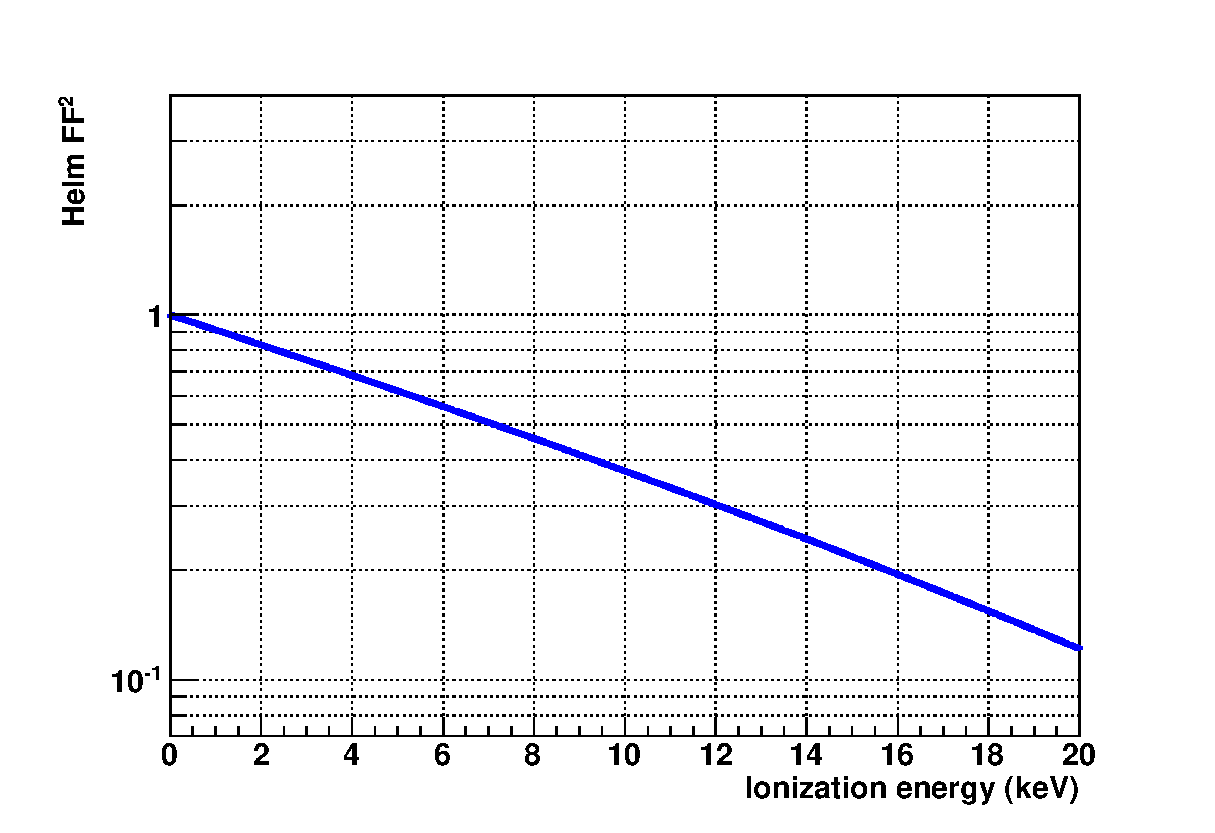
\includegraphics[width=0.7\textwidth]{HelmFormFactor}
			\caption[A plot of the Ge form factor versus ionization energy]
			{A plot of the Ge form factor versus ionization energy.  For a discussion of the 
			conversion from nuclear recoil energy to ionization energy, see 
			Section~\ref{sec:ResultsQuenching}.}
			\label{fig:HelmFF}.
		\end{figure}
	\section{Quenching}
	\label{sec:ResultsQuenching}
In ionization detectors, the calibration relating the energy deposited per amount of charge collected is generally performed by using gamma lines from a known source.  However, since photons interact by recoiling off of electrons in the detector, this calibration is only valid for other processes which deposit energy in a similar manner.  In contrast, a process that deposits energy in a detector by recoiling off of a nucleus (such as a WIMP interaction) does not generate the same amount of charge per amount of energy deposited as an electron-recoil interaction.  The relationship between the `seen' ionization from a nuclear recoil and the `seen' ionization from an electron recoil at the same energy is referred to as quenching.  For ionization detectors, a theory has been developed by Lindhard et al.~\cite{Lindhard:1961fa} to parameterize this relationship:

		\begin{equation}
			E_{ion} =  \frac{k E_{rec} g(\epsilon)}{1 + k g(\epsilon)}
			\label{eqn:LindhardFunction}
		\end{equation}
with 
		\begin{eqnarray*}
			g(\epsilon) & = & 3 \epsilon^{0.15} + 0.7\epsilon^{0.6} + \epsilon \\		
			\epsilon & = & 11.5 E_{rec} Z^{-7/3} \\
		\end{eqnarray*}
For germanium detectors, the constant, $k$, has been recently measured as 0.2 by Barbeau, et al.~\cite{Barbeau:2009fk}.  In a single-mode readout detector (e.g.~reading out \emph{only} ionization), nuclear recoil and electron recoil events are indistinguishable and so it is necessary to transform all theoretical spectra defined in recoil energy to ionization energy.  Unfortunately, accomplishing this requires inverting the Lindhard equation which is impossible to do analytically and so it essential to either obtain it numerically or to estimate this function with another function.  The function $E_{ion} =  \alpha E_{rec}^{\beta}$ provides an excellent approximation to this equation and can be easily inverted and differentiated.  Results from a fit of this function to the Lindhard equation (Eqn.~\ref{eqn:LindhardFunction}) for germanium detectors are shown in Figure~\ref{fig:LindhardFitResults}.  Fit values for $\alpha$ and $\beta$ are $0.204971$ and $1.13615$, respectively.

		\begin{figure}
			\centering
			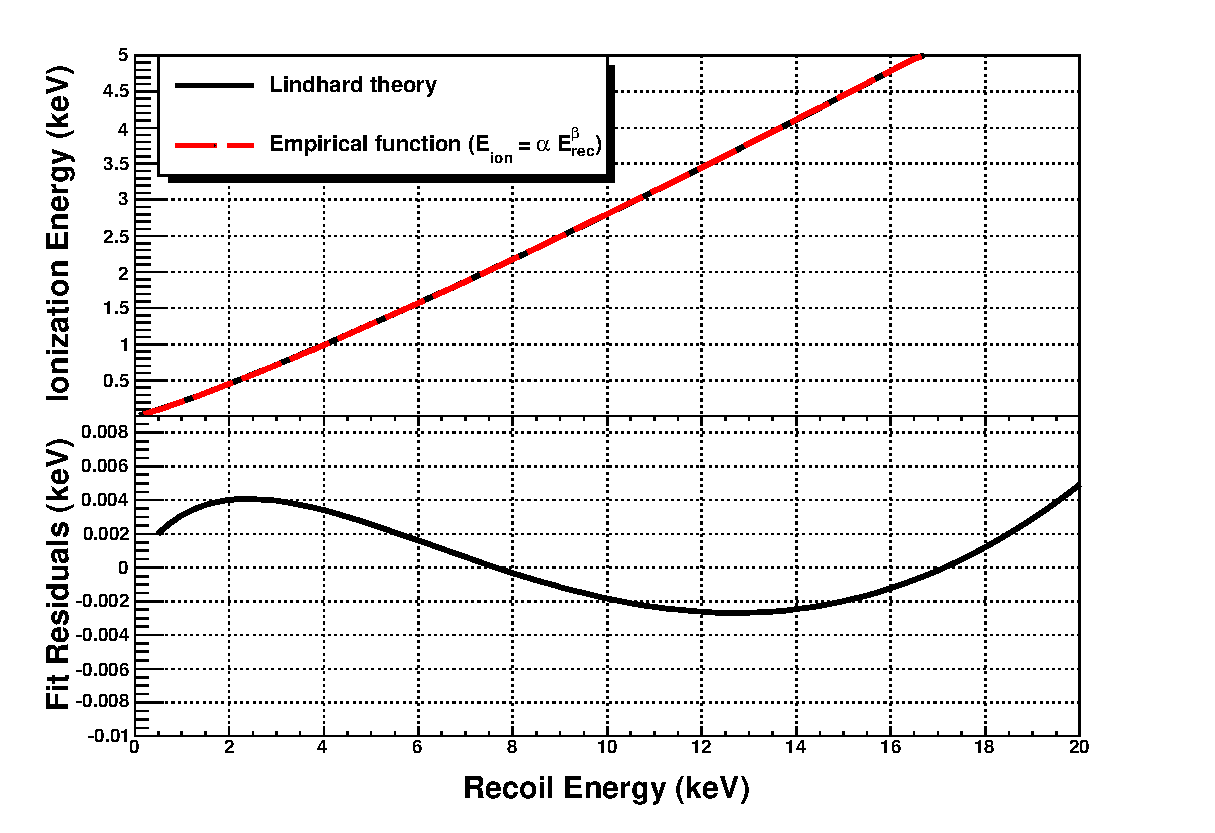
\includegraphics[width=0.7\textwidth]{quenching}
			\caption[Lindhard function with a fit to $E_{ion} =  \alpha E_{rec}^{\beta}$]
			{Lindhard function with a fit to $E_{ion} =  \alpha E_{rec}^{\beta}$.  
			The bottom plot displays the residuals, 
			indicating that the estimating function is good to better than 1\% in the 
			ionization energy range 0.5$\to$3.5~keV.}
			\label{fig:LindhardFitResults}
		\end{figure}
Combining this all together to determine the WIMP time and energy spectrum in terms of ionization energy yields the final differential rate:
		\begin{equation}
				\frac{dR}{dE_{ion}}  = \left(\frac{dR}{dE_{rec}} \right) \left(\frac{dE_{rec}}{dE_{ion}} \right) F^{2}
			\label{eqn:FinalFitSpectrum}
		\end{equation}	
A summary of the parameters used is given in Table~\ref{tab:BeGeFitParameters}.  The effect of including the escape velocity and the form factor for a low-mass (10~GeV) WIMP is shown in Figure~\ref{fig:1DDMSignal} where $t=0$.  This plot demonstrates the importance of a low threshold for detecting low-mass WIMPs since the escape velocity effectively truncates the WIMP spectrum above a certain energy.  Therefore, count rates for low-mass WIMPs become negligible for detectors with high enough thresholds.  The small correction from the form factor can be seen as a reduction in the count rate.  An example two-dimensional (energy and time) WIMP spectrum is shown in Figure~\ref{fig:2DDMSignal}.  In both of these plots, the differential rate is divided by the WIMP-nucleus cross-section.

		\begin{table}
			\centering
			\caption[Summary of parameters used in the WIMP exclusion fits]
			{Summary of parameters used in the WIMP exclusion fits.}
			\label{tab:BeGeFitParameters}
			\smallskip
			\begin{threeparttable}
				\begin{tabular}{l r}
					\toprule
					Parameter & Value (unit) \\
					\midrule
					\multicolumn{2}{l}{\emph{Fit parameters}} \\
					Atomic Mass & 72.96 (amu) \\
					$\rho_{D}$  &  0.4 (GeV cm$^{-3}$) \\
					Average velocity, $v_{0}$ & 230 (km s$^{-1}$) \\
					DM escape velocity, $v_{esc}$ & 600 (km s$^{-1}$) \\
					Velocity of the earth, $v_{E_{0}}$ & 244 (km s$^{-1}$) \\
					%Variational velocity of the earth, $v_{E}_{1}$\footnote{Not used in this fit} & 15 km s$^{-1}$ \\
					Detector mass &  0.33, 0.4\tnote{a} (kg) \\
					Nuclear skin thickness $s$ & 0.9 (fm) \\
					\multicolumn{2}{l}{\emph{Data set limits}} \\					
					Threshold & 0.5 (keV) \\
					Max energy & 3.5 (keV) \\					
					\bottomrule
				\end{tabular}	
				 \begin{tablenotes}
				       \item[a] {The smaller mass value is used when rise-time cuts are applied, see 
				       Section~\ref{sec:RisetimeCuts}.}
			     	\end{tablenotes}
			\end{threeparttable}
		\end{table}
		\begin{figure}
			\centering
			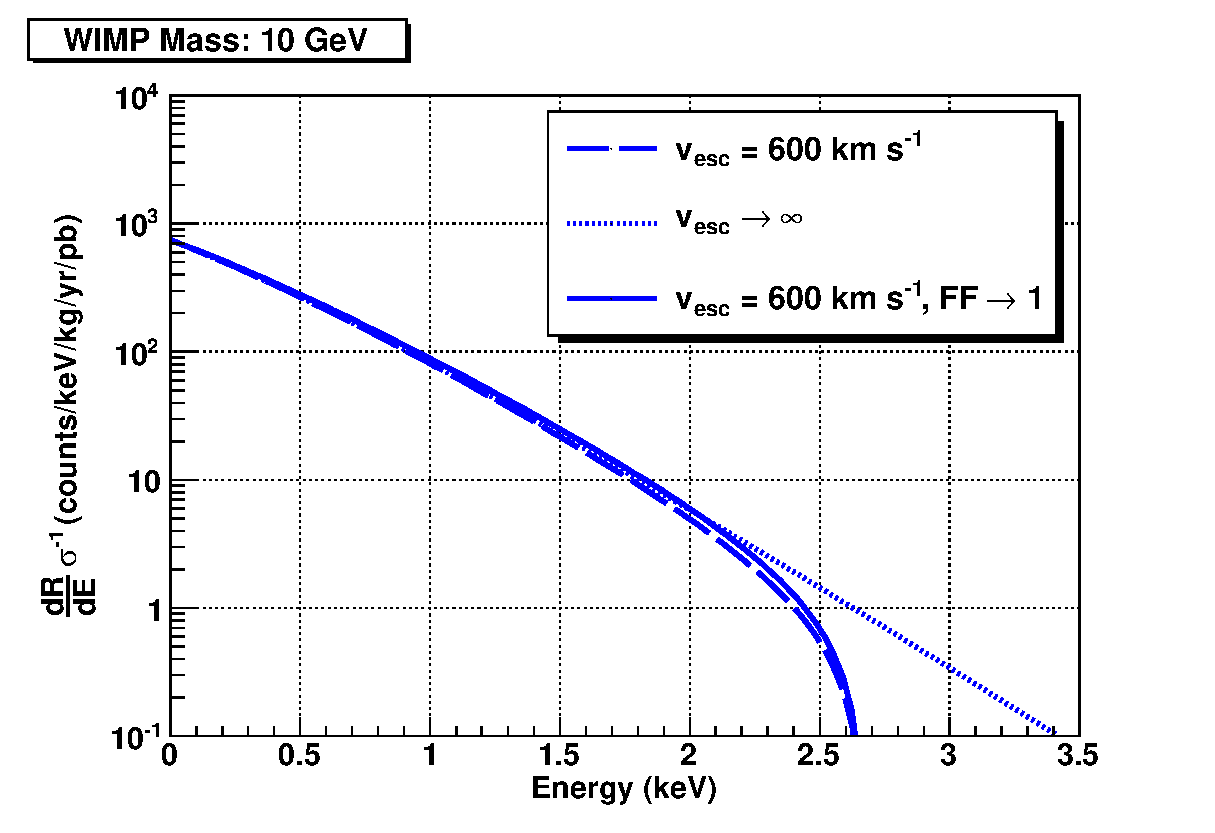
\includegraphics[width=0.9\textwidth]{WIMPMass10GeVExample}
			\caption[Count rate/cross section vs.~ionization energy for a 10~GeV WIMP]
			{Count rate/cross section vs.~ionization energy for a 10~GeV WIMP for 3 different model 
			variations: (1) Finite escape velocity and Helm form factor, (2) infinite escape velocity, 
			and (3) finite escape velocity and a form factor of 1.}
			\label{fig:1DDMSignal}
		\end{figure}
		
		\begin{figure}
			\centering
			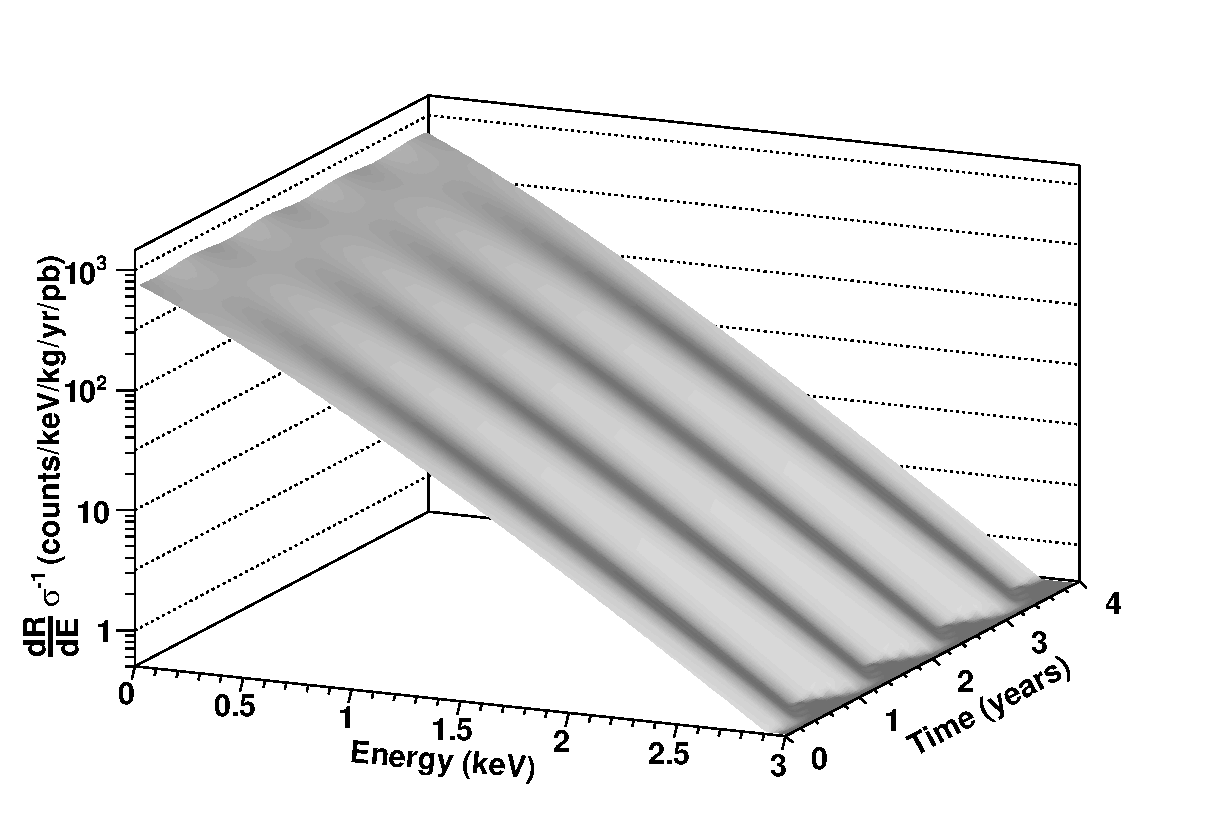
\includegraphics[width=0.9\textwidth]{WIMPModel}
			\caption[2-dimensional WIMP dark matter signal]
			{2-dimensional WIMP dark matter signal, $M_{WIMP} = $10~GeV.}
			\label{fig:2DDMSignal}
		\end{figure}


\section{Fit methodology} 

	The analysis of the \bege~data presented in the previous chapter, in particular Section~\ref{sec:BeGeLowEnergyFeatures}, uncovered several difficulties which must be addressed when determining limits with the data.  This section discusses the extraction of a signal limit using the maximum-likelihood method and explores the necessary mechanisms for dealing with unknown backgrounds.  
	
	\subsection{Obtaining limits using Maximum Likelihood}
	\label{sec:LimitsML}		

A maximum-likelihood analysis provides a mechanism for estimating the parameters of a model given a set of data.  There also exist standard techniques within the maximum-likelihood framework for hypothesis testing or searching for and generating limits on a signal that may exist in the data set.  In contrast to using $\chi^{2}$-minimization for parameter estimation, maximum likelihood does not require the binning of data
% though it does accommodate it
 and it does not provide a mechanism for estimating the goodness-of-fit.  The procedure for determining the set of parameters which best describes a data set involves constructing a likelihood function as the following:
		\[
		L = \prod^{n} f({\tbf}, x_{n})
		\]
where $f(\theta, x)$ is a probability distribution function (pdf) describing the data, $x_{n}$, with parameter set $\tbf$.  The true values of the parameters, $\boldsymbol{\theta_{T}}$, are then estimated by maximizing $L$, or, equivalently, by minimizing $-\log L$.  For some more-trivial pdfs, it is possible to find an analytical solution to the equation set: $-\frac{\partial ( \log L )}{\partial\tbf} = 0$, but normally the minimization of the function is handled numerically.  

Hypothesis testing defines a mechanism by which one compares two models to the same data to find the favored model.  It is useful when searching for limits on a signal since one can compare the null hypothesis (no signal) versus the model with signal included.  Hypothesis testing using likelihood functions is performed by using a profile-likelihood test which involves the construction of a profile-likelihood function over a parameter or set of parameters, $\theta_{0}$:
		\[
		\lambda(\theta_{0}) = \log L_{max}  - \log L_{max}(\theta_{0}, \boldsymbol{\theta_{n}})
		\]
assuming that $\theta_{0}$ is a subset of $\tbf$, or $\tbf = \{\theta_{0}, \boldsymbol{\theta_{n}}\}$.  $L_{max}$ is the likelihood function maximized for all parameters, and $ L_{max}(\theta_{0}, \boldsymbol{\theta_{n}})$ is the likelihood function at parameter value $\theta_{0}$ maximized over all other parameters except $\theta_{0}$.  The profile-likelihood function, $\lambda$ is asymptotically distributed according to a $\chi^{2}$ distribution with number-of-degrees-of-freedom (NDF) equal to the dimensionality of $\theta_{0}$, so that:
		\[
		2 \lambda (\theta_{0}) \sim \chi^{2}_{dim(\theta_{0})}
		\]
  This relationship can be used to determine a confidence interval for $\theta_{0}$.		

To demonstrate this methodology, consider the search for a signal, $S$, in some background with distribution, $B$, so that the log-likelihood function is
		\[
		-\log L (\alpha, \boldsymbol{\beta}) = -\sum^{n} \log (\alpha S (x_{n}) + B(\boldsymbol{\beta}, x_{n}))
		\]
where we have assumed that the only variable parameterizing the signal, $S$, is its amplitude, $\alpha$.  The true values of the model parameters are estimated by maximizing $L$ to obtain $\alpha_{0}$ and $\boldsymbol{\beta_{0}}$.  The upper and lower limits of $\alpha$ are then determined by finding the values $\alpha_{upper}$ and $\alpha_{lower}$ so that $\lambda(\alpha_{0} + \alpha_{upper}) =  P_{\chi^{2}_{1}} (CL)/2 = \lambda(\alpha_{0} - \alpha_{lower})$.  $P_{\chi^{2}_{1}} (CL)$ is the $\chi^{2}$ quantile for 1 degree-of-freedom at the CL (confidence level) percentage.  For example, if we assume a confidence level of 90\%, we solve the equations $\lambda(\alpha_{0} + \alpha_{upper}), \lambda(\alpha_{0} - \alpha_{lower}) = 2.71/2$ to find $\alpha_{lower}$ and $\alpha_{upper}$.  Typically, these solutions are found by scanning the parameters of interest  ($\alpha$ in this case) in the profile-likelihood function around the global extremum on a grid size determined by the desired precision.  More information regarding the profile-likelihood method and calculating confidence intervals with it can be found in~\cite{Venz1988}.

	\subsection{Obtaining limits in the presence of unknown backgrounds}
	\label{sec:LimitsUnknownBackgroundML}	
	
In some experiments it is sometimes difficult or impossible to determine precisely the background contamination in a region-of-interest for a signal.  This could arise for several reasons: e.g.~(1) poorly understood systematics from simulation, (2) overlapping signal and background in the region of interest, or (3) the inability to perform independent measurements of background by, for example, performing background-only data runs.  Especially in dark matter experiments, some or all of these could present an issue when attempting to understand data and generate limits on potential signals.  This is largely due to several factors, including that detectors looking for dark matter might operate at or close to their noise limits in poorly understood regions (e.g.~near threshold), signal can not be `turned off' to get a pure-background measurement, and simulations in low-energy regions might not offer precise estimates of backgrounds.  Several methods have been proposed to deal with poorly understood or unknown backgrounds, including the Maximum-gap method described in~\cite{Yell02} and a method proposed by Rolke et al.~\cite{Rolke2001} to treat the uncertainties in the background as statistical errors.  These methods are generally applicable to experiments with very low count rates in the signal region.  A method used by the CRESST experiment~\cite{Anglo2002} proceeded by initially fitting the spectrum to an empirically determined function using maximum likelihood and then using a profile-likelihood-like technique to determine the exclusion on a WIMP signal.  Another method similar to the CRESST method but with deeper numerical study has been proposed by Rolke et al.~to handle uncertainties in background by using a profile-likelihood technique~\cite{Rol05}.  The Rolke method is used in this analysis.  

The Rolke method treats the background as a nuisance parameter in the likelihood analysis, essentially using the data to estimate both the background and the signal simultaneously.  The technique itself is roughly equivalent to the profile-likelihood method, but accommodates boundary cases such as when the best estimate of a parameter constrained to be greater than 0 (e.g.~as in the case of a cross-section or number of counts) is less than 0, or when the likelihood function has no maximum as is the case when the signal and background look very similar or the number of data seen is less than that expected in background.  Rolke et al.~presented two techniques for dealing with these issues: an unbounded-likelihood method and a bounded-likelihood method; this analysis makes use of the latter.  The bounded-likelihood method is no different than the profile-likelihood method if the best fit of the parameter is in a physical or `acceptable' region.  However, if the best-fit parameter moves into an unphysical region, then the parameter is forced to its nearest physical boundary and the maximum likelihood is set as the value of the profile likelihood at that boundary.  

This can be made more clear by considering the example in Section~\ref{sec:LimitsML}:  In this example, $\alpha$ must be greater than or equal to 0 since a negative background has no physical meaning.  However, it is possible that a best fit can yield an estimate for $\alpha$ of $\alpha_{0}<0$.  In this case, $\alpha_{0}$ would be quoted as 0 and, for purposes of calculating an upper limit, $L_{max}$ would be replaced with the likelihood function $L$ maximized at $\alpha = 0$.  This can be summarized with the following equations:
		\begin{equation}
			\begin{array}{rcl}
				\alpha_0^{\prime} & = & \alpha_0 H (\alpha_0) \\
				\lambda' (\alpha) & = & \lambda(\alpha) - \lambda(\alpha \to 0) (1 - H(\alpha_0))
			\end{array}
		\end{equation}
where the primed values are used in the bounded-likelihood method and $H(x)$ is the Heaviside step function.  In this formalization, it is clear that the primed variables become the original unprimed variables for $\alpha_{0}\geq0$.  The upper limit on $\alpha$ is calculated similarly as before by increasing $\alpha$ until the profile likelihood, $\lambda'(\alpha)$, reaches the value of the desired $\chi^{2}$ quantile. 

 Especially when the parameters of the fit are near or at their boundaries, it is not ensured that $\lambda'$ follows a $\chi^{2}$ distribution and so it is essential to perform Monte Carlo studies to investigate the coverage of this technique for a particular model.  This can be done, for example, by the following:
		\begin{itemize}
			\item Scan the allowed parameter space of a model, 
			generating a data set at each point in parameter space via Monte Carlo
			\item Perform a likelihood analysis using the Rolke method, calculating limits at an 
			assumed confidence level, $CL$
			\item Determine if the calculated limits include the `true' value(s) (i.e.~those values of 
			the model used to generate the data set) of the parameter(s) of interest 
			\item Repeat many times to measure how often the calculated limits include the true values
		\end{itemize}			
% FixME JFW: I'm not sure I understand this sentence?    Doesn't one use the MC method above to actually generate the CL?
In essence, this is a guess-and-check test: one initially \emph{assumes} that the profile likelihood follows a $\chi^{2}$ distribution and then performs tests to ensure that it in fact does.  A model is over covered if the percentage of times the calculated limits include the true values is greater than $CL$ and is under covered if the opposite is true.  Rolke et al.~provide several concrete models where they demonstrate that their technique properly covers the model parameter space, i.e.~that the calculated coverage is at least the expected $CL$.  In practice, determining and scanning the allowed parameter space for coverage tests is difficult: for this analysis, this is discussed in Section~\ref{sec:LimitsCoverageTests}.


\section{Dark matter limits using data from a low-background \bege~detector at Soud\-an Underground Laboratory} 
\label{sec:DMLimitsWithSoudan}

	The data described and analyzed in Chapter~\ref{chap:AnalysisBeGe} were used to calculate limits on light dark matter following the procedures outlined in previous sections.  This section describes the data and model used during fitting and explores difficulties that arose during generation of these results.  Several systematic tests were performed to investigate how details of the fitting procedure might affect the results.  For systematic tests, a smaller subset of the data with $\sim$2~months of live-time was used, however the conclusions derived from this limited data set remain valid when considered for the entire data set.

	\subsection{Data and model}
	\label{sec:LimitsDataAndModel}	

The likelihood fitting was performed using the RooFit~\footnote{See \url{http://roofit.sourceforge.net/}.} framework developed by Wouter Verkerke and David Kirkby within the ROOT analysis package~\cite{Bru97}.  RooFit provides an abstract framework to perform different types of fitting, including both binned and unbinned maximum likelihood as well as chi-square minimization.  The package includes a set of pdfs from which one can construct more complex models and enables the user to generate his or her own models which could not have otherwise been constructed from the provided building blocks.  A toolkit extension was built within the RooFit framework including several pdfs of WIMP interactions.  More information on this constructed WIMP fitting framework can be found in Section~\ref{sec:WIMPPDFs}.  RooFit takes the built pdf models, automatically normalizes them, and constructs the appropriate negative log-likelihood or $\chi^{2}$ function which can then be minimized using numerical algorithms (i.e.~Minuit~\cite{James:1975dr}).


The likelihood function for the fit was constructed from the following pdfs (normalization not shown):	
		\begin{itemize}
			\item Flat background --  $f_{flat}(E) = 1$
			\item Exponential background --  $f_{exp}(E) = \exp\left(c_{1} E\right)$				
			\item Ge L-capture line -- $f_{Ge}(E) = \frac{1}{\sigma_{Ge}\sqrt{2 \pi}} 
								\exp\left(-\frac{(E - \mu_{Ge})^{2}}{2 \sigma_{Ge}^{2}}\right)$
			\item Zn L-capture line -- $f_{Zn}(E) = \frac{1}{\sigma_{Zn}\sqrt{2 \pi}} 
								\exp\left(-\frac{(E - \mu_{Zn})^{2}}{2 \sigma_{Zn}^{2}}\right)$				
								
			\item WIMP pdf -- $f_{WIMP}(E) = $Function~\ref{eqn:FinalFitSpectrum}				
		\end{itemize}			
These pdfs were combined additively, each with an associated parameter -- $N_{flat}$, $N_{exp}$, $N_{Ge}$, $N_{Zn}$, $N_{WIMP}$  -- measuring the number of events in each distribution.  The sum of these parameters, $\sum N_{x}$, was included in the likelihood function so that the final extended likelihood function (with each pdf, $f_{x}$, automatically normalized over the range of the fit) was:
		\begin{equation}
			- \log L = -\log \left( f_{Pois} \left( \sum_{x} N_{x}, N_{obs} \right) \right) 
					- \sum_{i} w_{i} \log \left( 
						\frac{1}{\sum_{x} N_{x}} 
							\left( \sum_{x} N_{x} f_{x} (E_{i})
							\right) 
						\right)
		\end{equation}
where the sums over $x$ are over the pdfs in the distribution, the sum over $i$ is over each data point or bin, and $w_{i}$ is the weighting for a particular data point with $N_{obs} = \sum_{i} w_{i}$.  The weight of each event, $i$, is determined by the inverse of the total efficiency function (see Section~\ref{sec:BeGeLowEnergyFeatures}) at the energy of the event, $E_{i}$.  The formalization of the WIMP pdf in Equation~\ref{eqn:FinalFitSpectrum} actually provides counts/kg/keV/day and so the number of counts, $N_{WIMP}$, in this pdf is not an independent parameter but rather equal to the integration of $f_{WIMP}$ over the fit energy range multiplied by the time of the experiment and the mass of the detector.  This meant that $N_{WIMP}$ was proportional to the WIMP-nucleus cross section, $\signuc$, and so constraints on the number of WIMP interactions directly related to a limit on the cross section.  Therefore, the profile-likelihood function for $\signuc$, $\pll$, was calculated directly.  The mass of the WIMP, $M_{W}$ is also a free parameter which defines the shape of the distribution.  To determine limits on $\signuc$ for a range of WIMP mass values, $M_{W}$ was stepped through a range from $\sim4\to100$~GeV, calculating limits on $\signuc$ at each mass value.  

The mean values of the L-capture lines ($\mu_{Zn}, \mu_{Ge}$) were fixed (1.1 and 1.299~keV) and the sigmas ($\sigma_{Zn}, \sigma_{Ge}$) were fixed according to the empirically determined resolution function from Equation~\ref{eqn:SigmaEqn}.  All other parameters were allowed to float, though the numbers of the flat and exponential background, $N_{exp}, N_{flat}$, were constrained greater than or equal to 0 and the shape parameter, $c_{1}$, of the exponential was allowed to float only slightly positive.  A summary of the parameters and their ranges is given in Table~\ref{tab:WIMPFitParameterRanges}. 
		\begin{table}
			\centering				
			\caption[Allowed ranges and values of parameters used in the WIMP fit]
			{Allowed ranges and values of parameters used in the WIMP fit.  Limits were chosen to avoid obtaining best-fit 	
			parameters near limit boundaries.  Therefore, some parameters -- e.g.~cross sections -- were allowed to float to 
			unphysical regions.}
			\label{tab:WIMPFitParameterRanges}
			\smallskip
			\begin{threeparttable}
				\begin{tabular}{l c r }
				\toprule
				Parameter & Range & Unit \\
				\midrule
				Ge L-capture mean, $\mu_{Ge}$ & 1.299 (fixed) & keV \\
				Ge sigma, $\sigma_{Ge}$ & 7.55$\times10^{-2}$ (fixed) & keV \\				
				Zn L-capture mean, $\mu_{Ge}$ & 1.1 (fixed) & keV \\
				Zn sigma, $\sigma_{Ge}$ & 7.48$\times10^{-2}$ (fixed) & keV \\
				WIMP-nucleus cross section, $\signuc$ & $-10\to100$\tnote{a} & pb \\
				Exponential shape parameter, $c_{1}$ & $-100\to5$ & keV$^{-1}$ \\				
				$N_{flat}$ & $0\to10^{5}$ & counts \\			
				$N_{exp}$ & $0\to10^{5}$ & counts \\	
				$N_{Ge}$\tnote{b} & $0\to10^{5}$ & counts \\			
				$N_{Zn}$\tnote{b} & $0\to10^{5}$ & counts \\						
				\bottomrule
				\end{tabular}		
				 \begin{tablenotes}
				       \item[a] {The upper limit was expanded dynamically to ensure that $\pll$ would exceed
				       the desired $\chi^{2}$-quantile value.}
				       \item[b] { For fits when the relative amplitude of the two L-lines was constrained, these two 
				       parameters became a single parameter with the same limits.}
			     	\end{tablenotes}
			\end{threeparttable}
		\end{table}
The inclusion of the exponential background in the null model was not due to any \emph{a priori} assumption or background simulation, but instead as a mechanism to quantify our agnosticism as to the source of 
this shape in % FixME JFW this contribution to?
the data.  The cause could be from several factors in indeterminate combination: (1) noise fluctuations -- deviations in noise could manifest as a widening of the noise pedestal (gaussian) which would appear exponential; (2) untagged microphonics -- microphonics can generate an exponential at low energies~\cite{Morales1992410}; (3) slow-rise-time-event contamination -- an incomplete rejection of slow events could induce this shape, see Section~\ref{sec:RisetimeCuts}; (4) other unknown environmental (electronic and/or temperature) variations; (5) low-mass WIMP interactions.  The source of this shape is discussed in more detail in Section~\ref{sec:BeGeLowEnergyFeatures}.  Only after all sources of background have been independently and conclusively measured can one determine a more precise background model to feed back into the likelihood function.  To generate limits using this data given our current state of knowledge, it must suffice to treat the shape and amplitude of this background as nuisance parameters and follow the prescription of Rolke et al.~\cite{Rol05} as described in Section~\ref{sec:LimitsUnknownBackgroundML}.  However, since the WIMP signal is almost indistinguishable from an exponential in energy space, the inclusion of an unconstrained exponential posed some difficulties during the fits; these and other difficulties are outlined in Section~\ref{sec:LLPathologies}.
Fits with different constraints and methodologies were performed to investigate systematics of the fit and to determine how different constraints affected the calculated limits.  Three main sets of fits were performed:
		\begin{itemize}
			\item Unbinned fit -- No additional constraints on parameters
			\item Binned fit -- A particular binning was chosen
			\item Fixed relative amplitudes of the Ge and Zn L-capture lines (with both binned and unbinned fits)
		\end{itemize}			
In each of these fit sets, exclusions were calculated using data with different cuts applied, including rise-time cuts of varying acceptance efficiency and microphonics cuts:
	\begin{enumerate}	
		\item Microphonics and LN-fill cuts
		\item Microphonics, LN-fill cuts \emph{and} one of: 40\%, 50\%, 60\%, 70\%, 80\%, 90\%, 95\%, and 99\%
		acceptance rise-time cuts.
	\end{enumerate}
These cuts and associated data are described in detail in Sections~\ref{sec:MicroCuts} and~\ref{sec:RisetimeCuts}.  The results of the different fit sets are outlined in Sections~\ref{sec:LimitsUnbinned} and~\ref{sec:LimitsConstrained}.  

	\subsection{Fit difficulties and likelihood-function pathologies}
	\label{sec:LLPathologies}
			
While performing the exclusion fits, a number of issues were encountered with the log-likelihood and profile-likelihood functions.  In particular, the profile likelihood did not always exhibit a parabolic shape due to three main reasons: (1) similarity of signal and background -- background (both exponential and flat) could be similar to a WIMP signal at certain WIMP masses; (2) parameters at bounds during the calculation of $\pll$; and (3) unconstrained background exponential shape, leading to local minima away from the global minima.  Examples of profile-likelihood functions are given in Figure~\ref{fig:FitPathologies} and will be referred to throughout this section.  These functions were generated with data with 99\% rise-time cuts applied and and unbinned fits performed with constraints on the relative amplitudes of the Ge and Zn L-capture lines (see Section~\ref{sec:LimitsConstrained}), but are exemplary of $\pll$ for all types of fits performed.  This data set and model combination has been used to generate all the example results in this section.
		
		\begin{figure}
			\centering
			\subfigure[WIMP masses 40$\to$100~GeV]{
				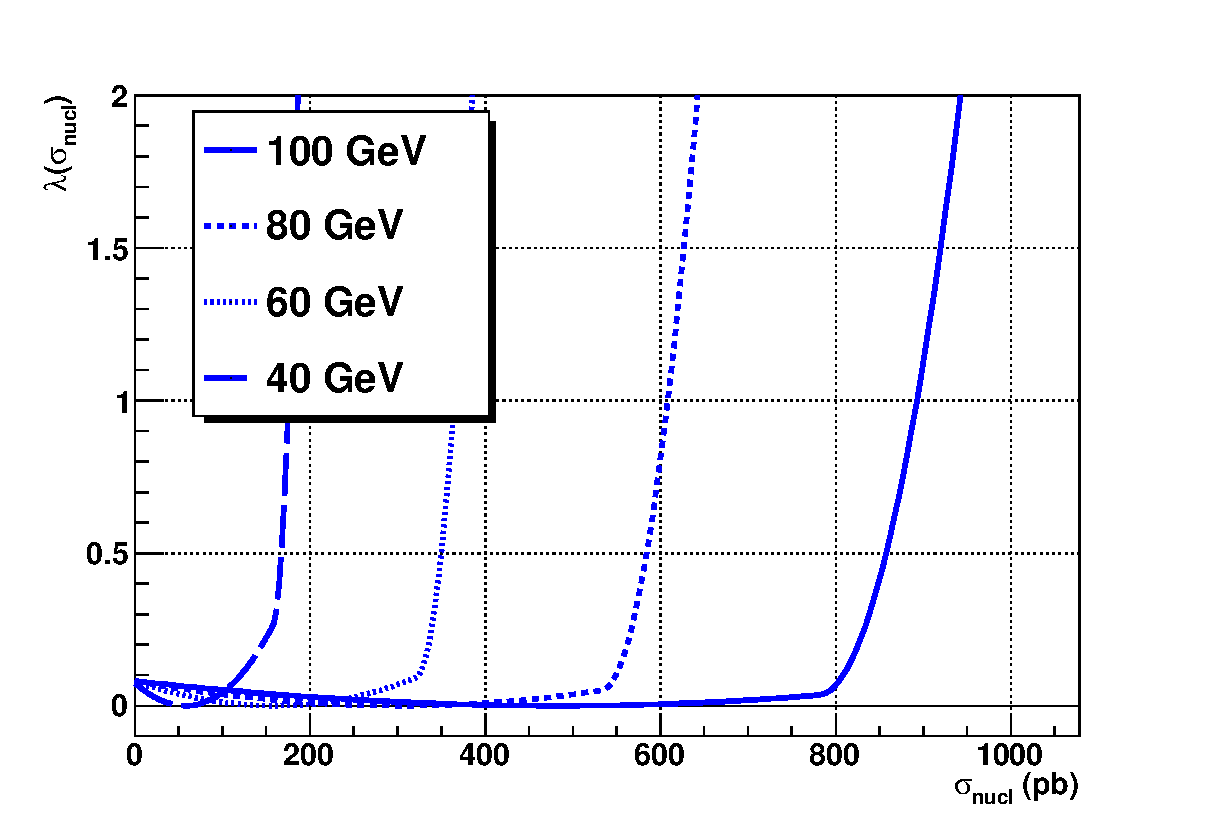
\includegraphics[height=0.4\textheight]{PLLCompare40.0}
				\label{fig:PLLRangeForty}
			}
			\subfigure[WIMP masses 4$\to$11~GeV]{
				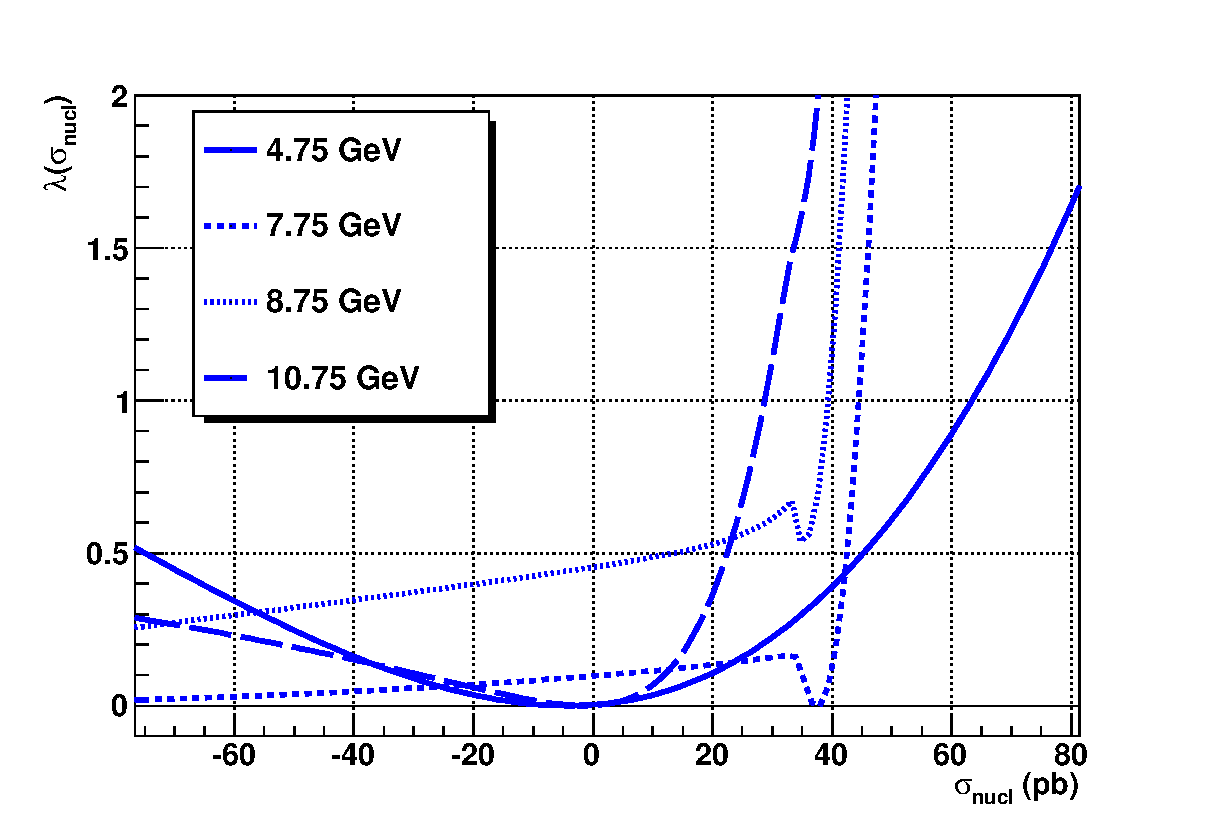
\includegraphics[height=0.4\textheight]{PLLCompare10.75}
				\label{fig:PLLRangeSeven}						
			}				
			\caption[$\pll$ for a range of WIMP Masses]
			{$\pll$ for a range of WIMP Masses.  See text for discussion of the shapes
			seen.}
			\label{fig:FitPathologies}
		\end{figure}
		
		\subsubsection{Signal, background similarity}
		\label{sec:LLPathoSBSimilarity}
			
			\begin{figure}
				\centering
				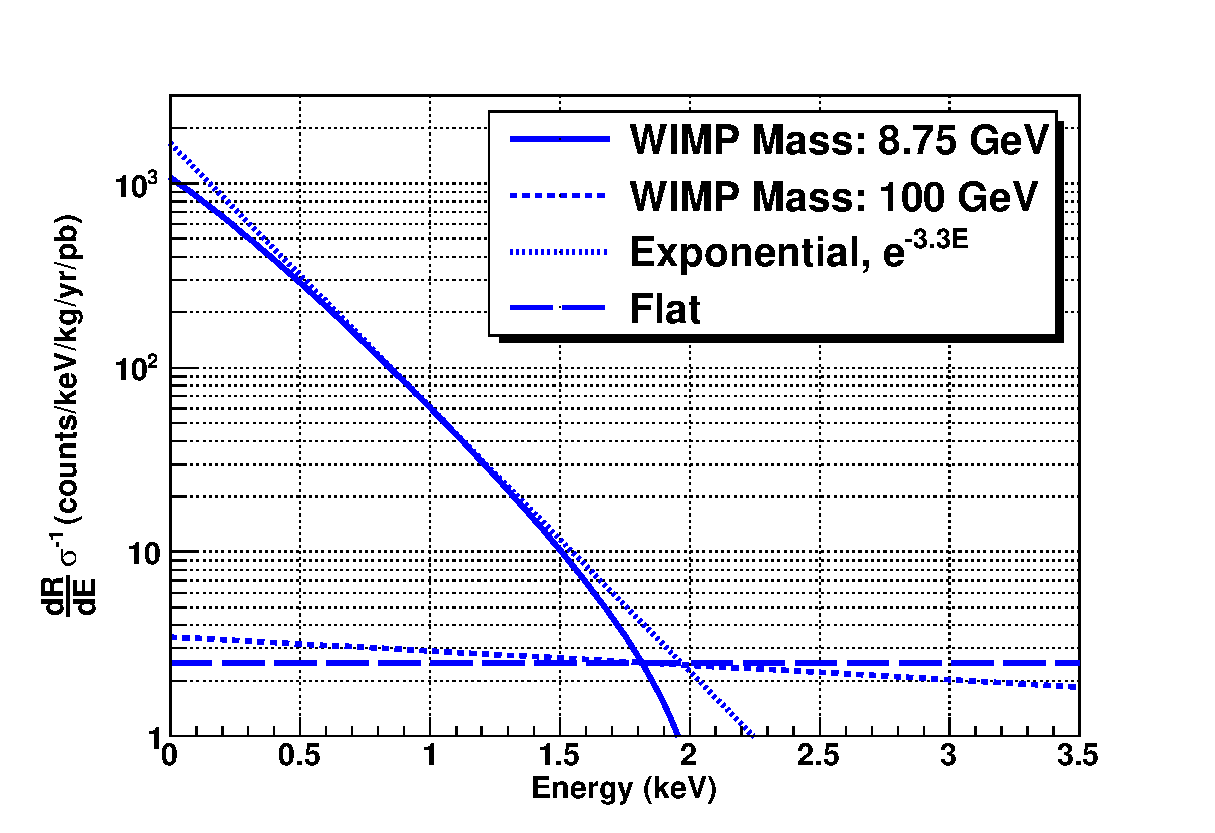
\includegraphics[width=0.9\textwidth]{WIMPModelCompare}
				\caption[Similarity of WIMP signal and background]
				{Similarity of signal and background, comparing the exponential and flat components of the background with a WIMP signal.  
				The shape parameter of the exponential function is set to -3.3 keV$^{-1}$, the best-fit value from data.  Flat and exponential backgrounds have 
				arbitrary normalizations for comparison to the WIMP signals.}
				\label{fig:SBSimilarity}
			\end{figure}			
			
			\begin{figure}
				\centering
				\subfigure[WIMP mass 100~GeV]{
					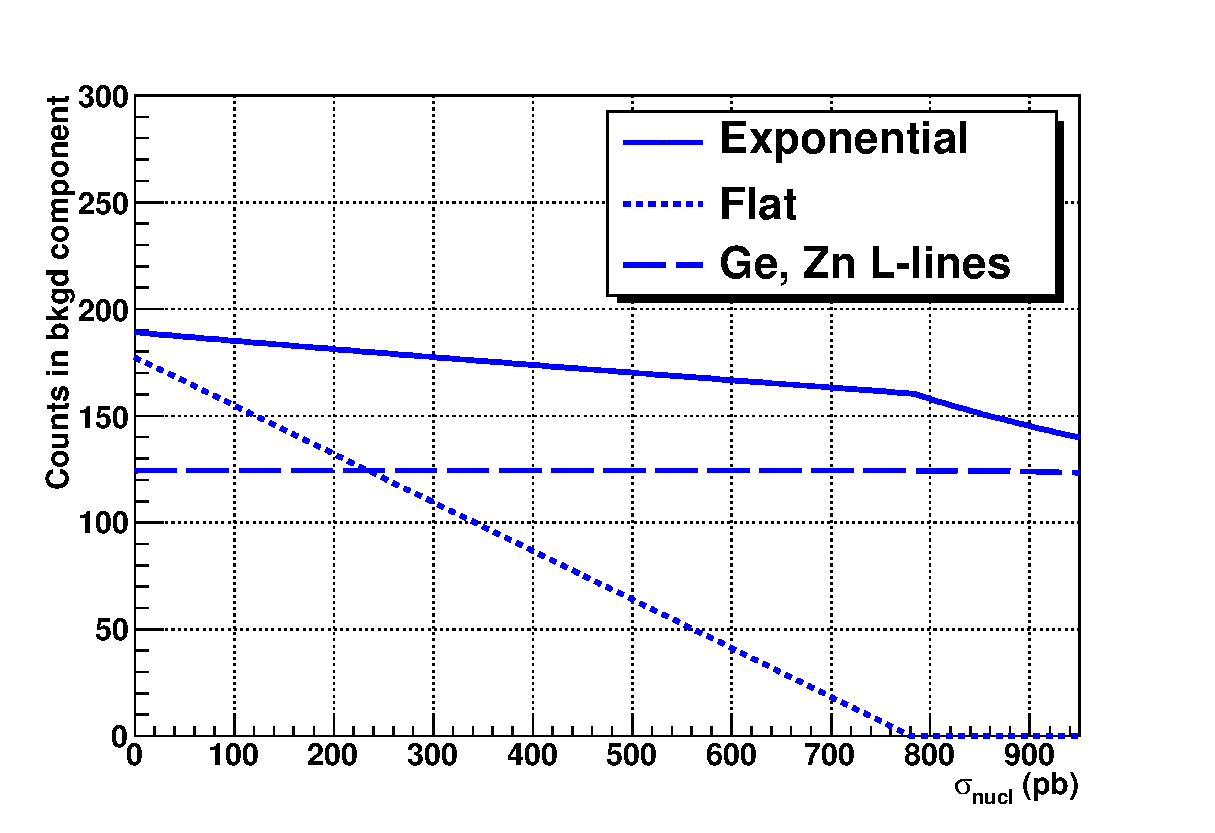
\includegraphics[height=0.4\textheight]{Summary100.0}
					\label{fig:SBCounts100}
				}
				\subfigure[WIMP mass 8.75~GeV, with zoom in on count region $0\to30$.]{
					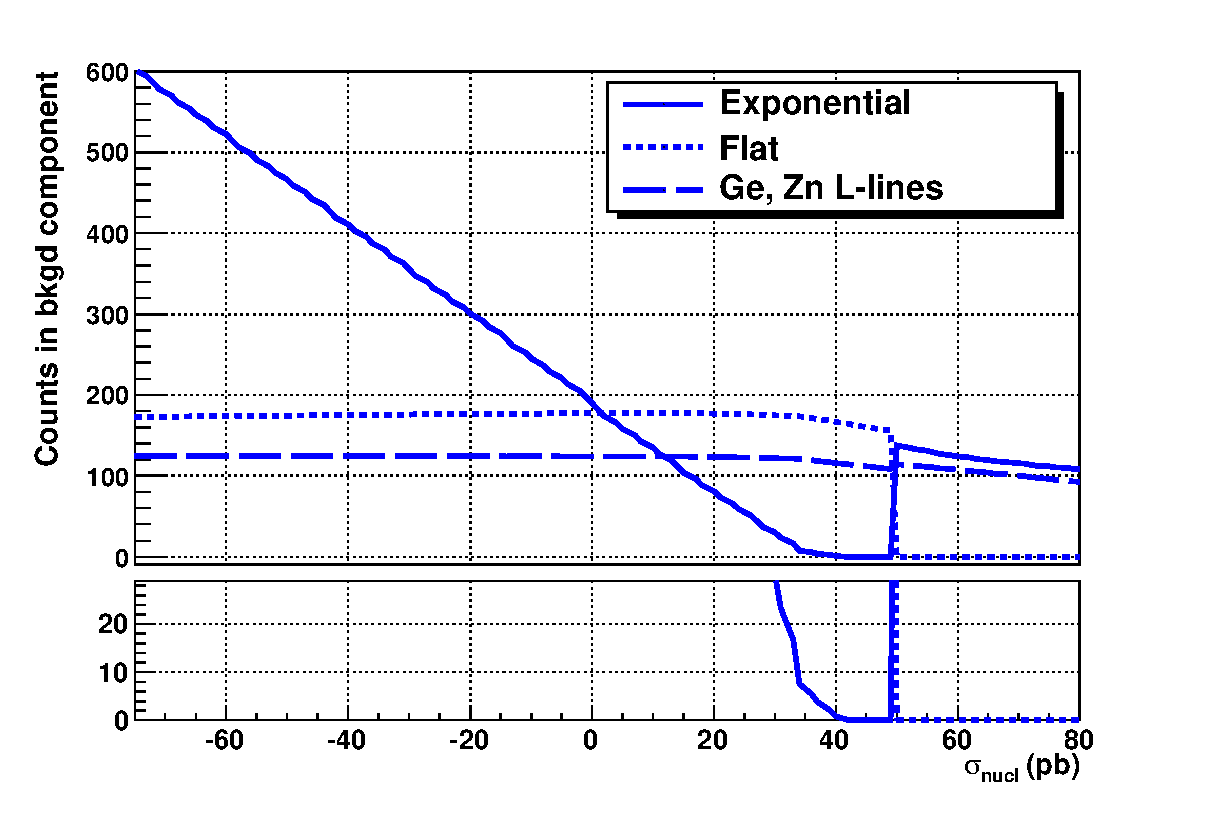
\includegraphics[height=0.4\textheight]{Summary8.75}
					\label{fig:SBCounts8.75}						
				}				
				\caption[Counts in background components versus $\signuc$]
				{Counts in background components versus $\signuc$.  The values of the 
				components are determined during a profile-likelihood scan of $\signuc$.}
				\label{fig:SBCountsInComponents}
			\end{figure}	
		
For certain values of WIMP masses, the background and 	signal can appear very similar.  This can be seen, for example, in Figure~\ref{fig:SBSimilarity} which is a plot displaying WIMP signals of $M_{W}=8.75$ and 100~GeV together with an exponential spectrum ($e^{-3.3 E}$, the best-fit shape parameter for the model without included WIMP signal to data with a 99\% rise-time cut applied) and a flat spectrum both with arbitrary normalization adjusted for comparison.  Because $\pll$ includes an implicit maximization of the likelihood for different values of $\signuc$, it is instructive to consider how the components of those fits depend on $\signuc$.  Figure~\ref{fig:SBCountsInComponents} includes two plots of counts in background components (flat, exponential and L-line amplitudes) versus $\signuc$, where the background components are the parameters which maximize the likelihood for a given value of $\signuc$.  %These plots can help us understand features in the likelihood functions.  
If we first consider Figure~\ref{fig:SBCounts100} ($M_{W}$ = 100~GeV), it is clear that L-line background components vary only slightly with $\signuc$ whereas the exponential and flat components vary almost linearly with the flat component changing more quickly than than the exponential component.  When the limit of the flat background is reached at 0, it generates a kink in the likelihood function visible in Figure~\ref{fig:PLLRangeForty}.  Generally, parameters are allowed to float beyond their physically-allowed values to avoid such features in the likelihood function.  However, due to the similarity of the signal and background it was found that the flat background component would continue decreasing if it were allowed to float below zero leading to a very flat profile-likelihood function.  The linear variation of the flat and exponential background components with $\signuc$ coupled with the relative independence of the other parameter indicates that the variation of $\pll$ is dominated by the extended parameter\footnote{It can be shown that a minimization of this term leads to a linear dependence between the counts and $\signuc$.  If other terms in $\pll$ contribute, then the relationship becomes non-linear.}: $-\log \left( f_{Pois} \left( \sum_{x} N_{x}, N_{obs} \right) \right)$.  Therefore, the upper limit on $\signuc$ calculated using the profile-likelihood method is essentially equivalent to calculating a poisson upper limit on true counts given number of counts seen, and assuming that all these counts come from signal.  %This equivalence gives confidence in this method.  

We can then consider lower WIMP mass (8.75~GeV) where the shape of the WIMP signal is roughly equivalent to the shape the exponential background component in the data.  The relevant plots for this are Figure~\ref{fig:SBCounts8.75} and Figure~\ref{fig:PLLRangeSeven}, focusing on $M_{W}$=8.75~GeV in the latter.  It is important to note the $\pll$ for this mass does not intersect 0 in Figure~\ref{fig:PLLRangeSeven}; this is because no minimum of the $-\log L$ was found in the scanned region for $\signuc$ and was therefore defined as the value of $-\log L$ at the lowest scanned value of $\signuc$ (-100~pb).  To define an upper limit with this function, the Rolke prescription outlined in Section~\ref{sec:LimitsUnknownBackgroundML} would be followed, defining the minimum of $-\log L$ to be at $\signuc$ = 0.  It is clear that, in contrast to the previous case with signal of a WIMP at $M_{W}$=100~GeV, the flat and L-line components of the background are largely independent of $\signuc$, whereas the exponential component varies almost linearly below 35~pb and reaches its lower bound of 0 around 40~pb.  (The transition region between 35 and 40~pb which manifests a local minimum will be discussed in the following section.)  As before, the linear variation indicates that the likelihood is dominated by the extended term because the signal and background have a roughly equivalent shape.  The transition at higher $\signuc$ (50~pb) is due to the exponential shape constant floating to  $\sim0$ and taking over the contributions from the flat component.  This can be seen in Figure~\ref{fig:FitExpoShapeVsSigma}.
	
		\subsubsection{Local minima of \texorpdfstring{$\pll$}{profile-likelihood function}}
		\label{sec:LLPathoLocalMinima}
			
			\begin{figure}
				\centering
				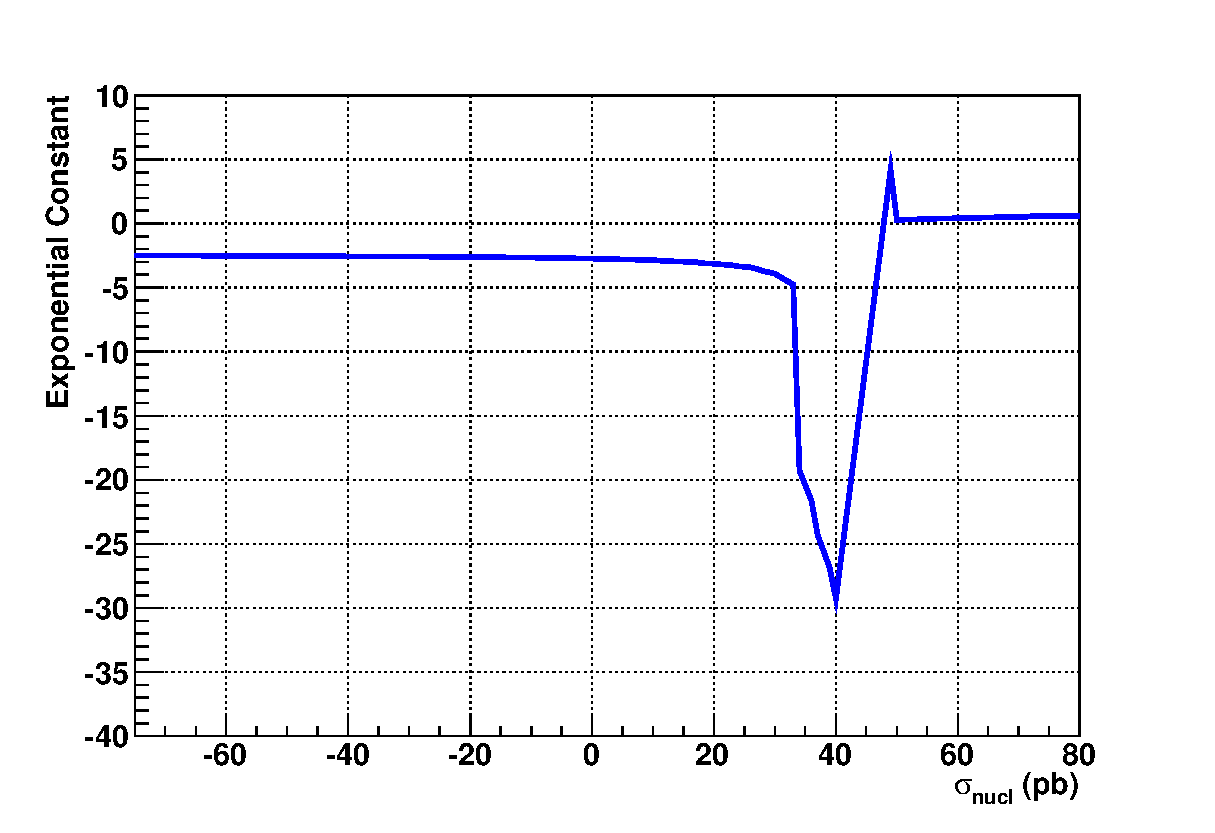
\includegraphics[width=0.9\textwidth]{ExpConst8.75}
				\caption[Exponential constant (shape parameter) versus $\signuc$]
				{Exponential constant (shape parameter) versus $\signuc$ for WIMP mass 8.5~GeV.
				The value of the exponential constant is determined during a profile-likelihood scan
				of $\signuc$.}
				\label{fig:FitExpoShapeVsSigma}
			\end{figure}
	
			\begin{figure}
				\centering
				\subfigure[$\signuc$ = 33.3~pb]{
					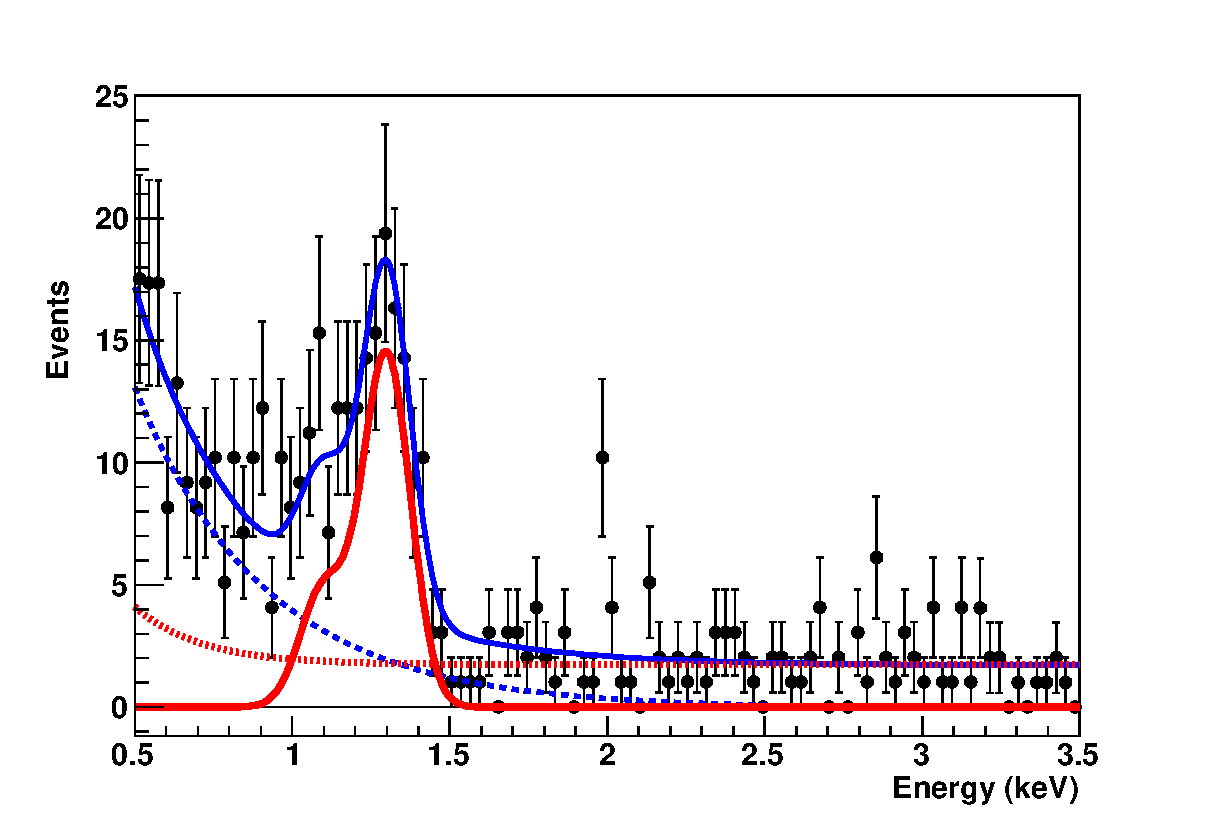
\includegraphics[height=0.36\textheight]{DataExclusionWIMPMass:8.75GeV33.3}
					\label{fig:ExpoFit33.3}
				}
				\subfigure[$\signuc$ = 34.8~pb]{
					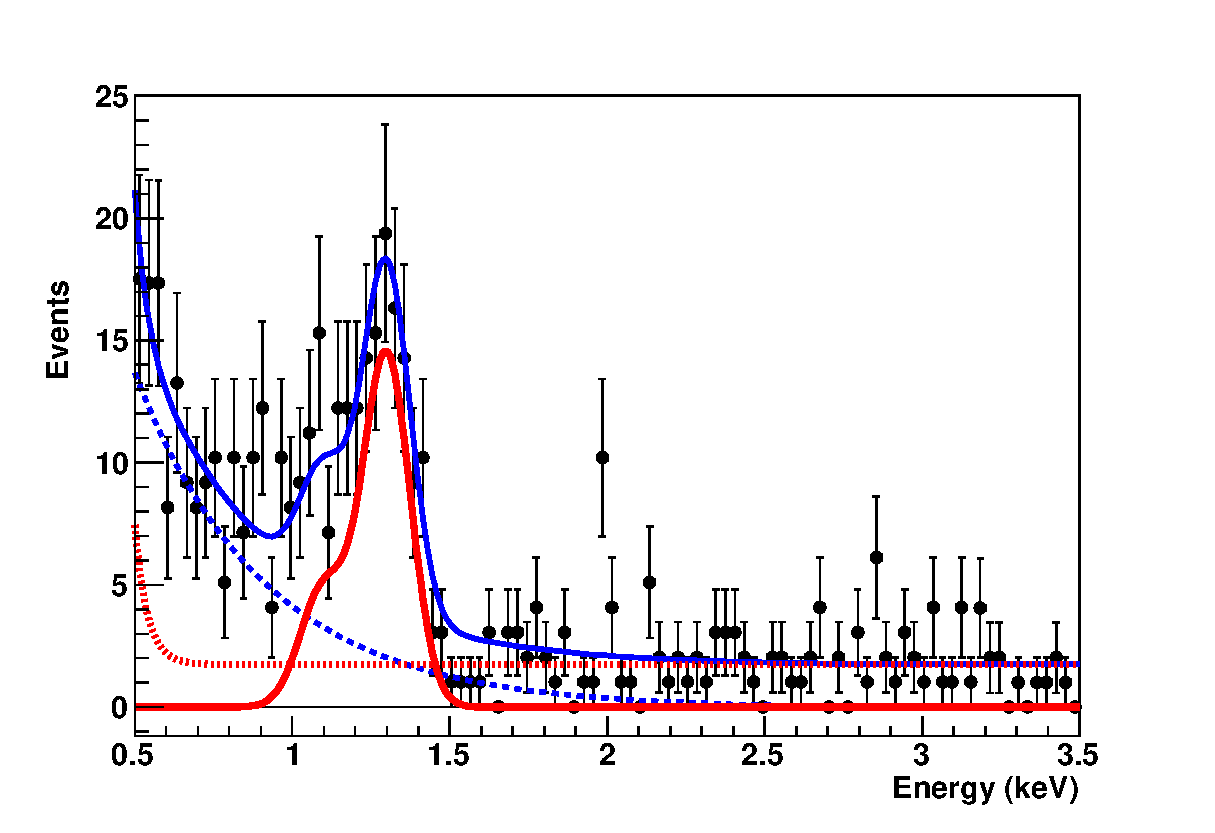
\includegraphics[height=0.36\textheight]{DataExclusionWIMPMass:8.75GeV34.8}
					\label{fig:ExpoFit34.8}						
				}					
				\caption[Abrupt changed of exponential background shape during fitting]
				{Example of how the exponential background shape changes abruptly during a profile 
				likelihood scan for a WIMP Mass of 8.75~GeV.  The separate components of the fit are shown: 
				WIMP signal (dashed), L-capture lines (solid), exponential + flat background (dotted), and the 
				sum (solid). }
				\label{fig:FitExpoFitExample}
			\end{figure}	

The $\pll$ for $M_{W}$ = 8.75~GeV in Figure~\ref{fig:PLLRangeSeven} includes a local minimum contained in the range $34\leq\signuc\leq40$~pb.  From Figure~\ref{fig:SBCounts8.75}, it is clear this feature does not arise from the exponential background being at its limit since the amplitude does not reach its lower bound until $\signuc>$40~pb.  Instead, this characteristic is due to the fact that the exponential shape parameter is allowed to float to very negative numbers, producing a background function sharply decreasing with energy.  (The lower limits of this parameter were kept low enough so that no fit would push the parameter to its bound.)  This can be seen clearly in Figure~\ref{fig:FitExpoShapeVsSigma} where the exponential shape parameter decreases sharply around 30~pb after remaining largely constant for lower values of $\signuc$.  A complementary set of plots in Figure~\ref{fig:FitExpoFitExample} provide a visualization of this abrupt change.  This issue occurred when the shape of the exponential background was very similar to the shape of the applied WIMP signal which meant, for example, that the affected WIMP mass range was different for fits generated with data with rise-time cuts applied and for fits made on data with only microphonics cuts applied.  In particular, the rise-time-cut data exhibited a sharper exponential decline (more negative exponential shape constant) than the microphonics-cut data yielding an affected range of $\sim$6-9~Gev versus 7-10.5~GeV, respectively.  The abrupt variations in the exponential shape parameter also induced features in exclusion plots for $\sigman$; these are discussed in Sections~\ref{sec:LimitsUnbinned} and~\ref{sec:LimitsConstrained}.

		\subsubsection{Conclusions}
		\label{sec:LLPathoConclusions}

The realization of several non-parabolic features underscores the care which must be taken when deriving limits from models with similar background and signal.  Some methods (e.g.~the HESSE functionality in MINUIT~\cite{James:1975dr}) estimate the error on the parameter by assuming a parabolic shape and extrapolating $\pll$ around its minimum by using the measured second derivative at the extremum.  For non-parabolic $\pll$ functions it is clear this won't work, and could possibly yield inappropriate bounds on $\signuc$.  For example, in Figure~\ref{fig:PLLRangeSeven} the $\pll$ for $M_{W}$ = 7.75~GeV indicates a minimum at $\sim$37~pb: a parabolic estimate of the the lower bound would be significantly non-zero %FixME, define what it *would* be?
whereas an estimate using the Rolke method would define the lower bound as 0!  Of course, as with all Frequentist methods it is essential to estimate the performance of the method using Monte Carlo tests; results of such an investigation are presented in Section~\ref{sec:LimitsCoverageTests}.

	\subsection{Coverage tests}
	\label{sec:LimitsCoverageTests}			

		\begin{sidewaysfigure}
			\centering
			\subfigure[4.25$\to$8.25~GeV]{
				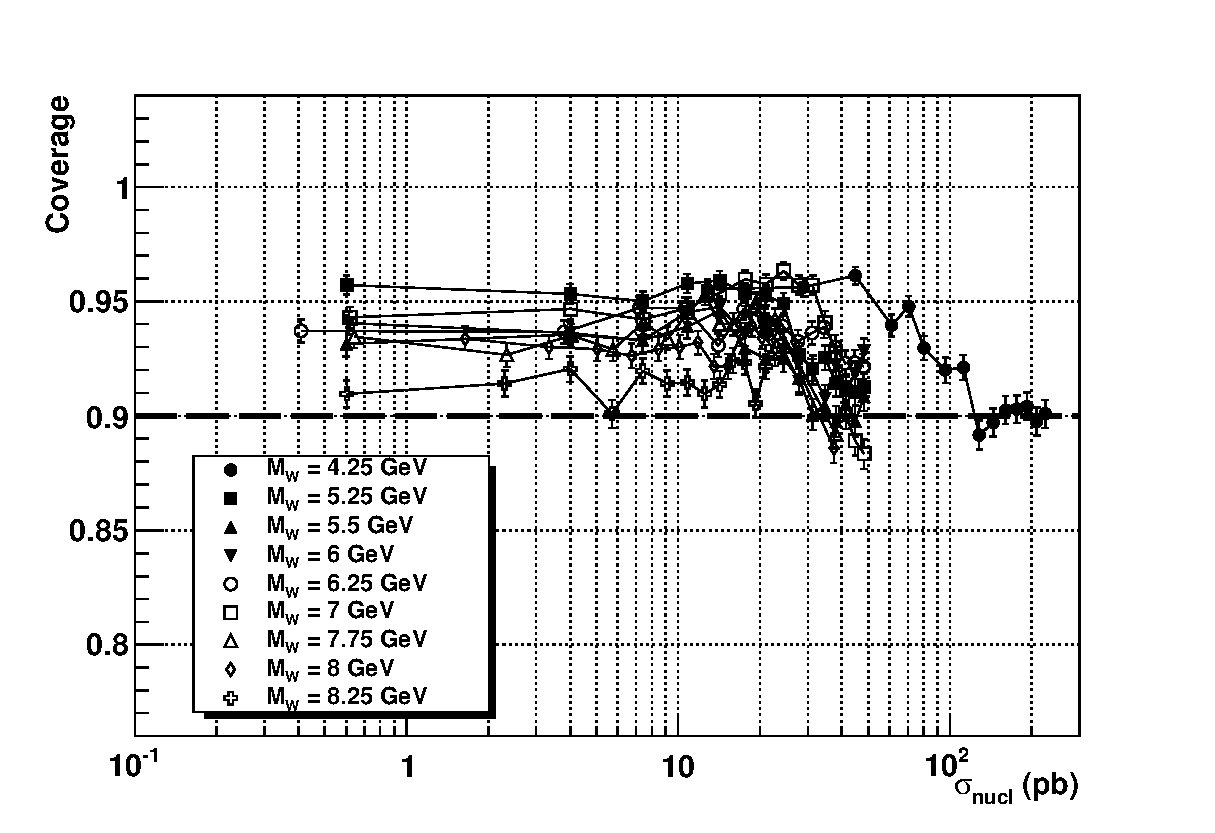
\includegraphics[width=0.46\textheight]{CoverageWithLastWIMP8.5}
				\label{fig:Coverage8.5}
			}
			\subfigure[8.5$\to$11~GeV]{
				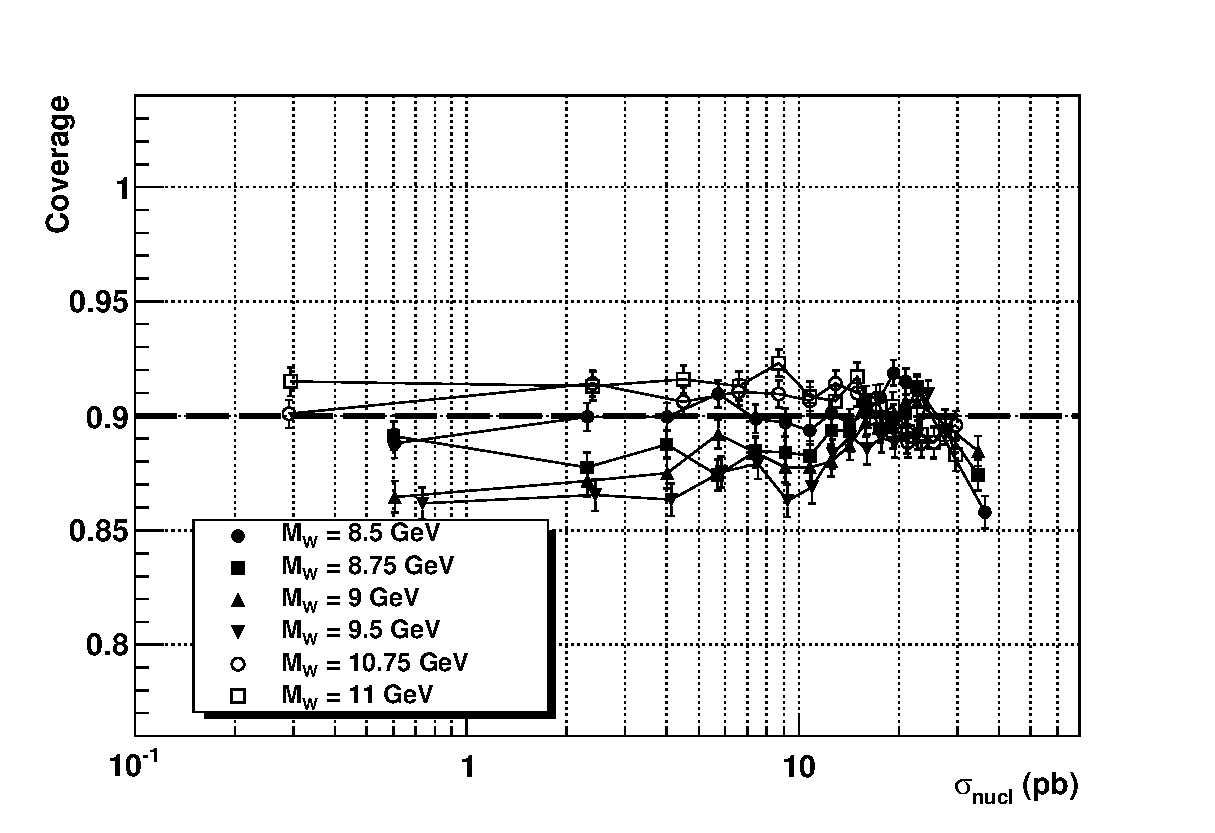
\includegraphics[width=0.46\textheight]{CoverageWithLastWIMP13}
				\label{fig:Coverage13}						
			}
			\subfigure[13$\to$22~GeV]{
				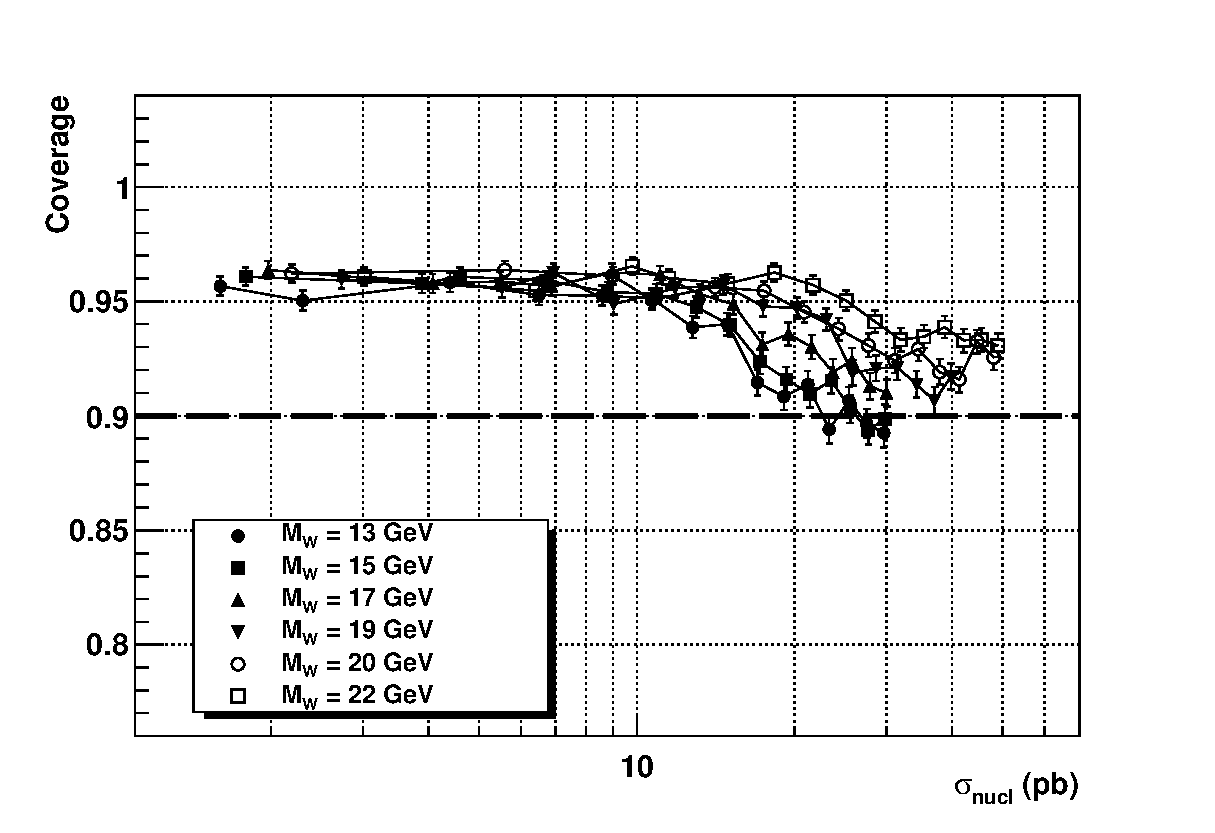
\includegraphics[width=0.46\textheight]{CoverageWithLastWIMP50}
				\label{fig:Coverage50}						
			}												
			\subfigure[50$\to$100~GeV]{
				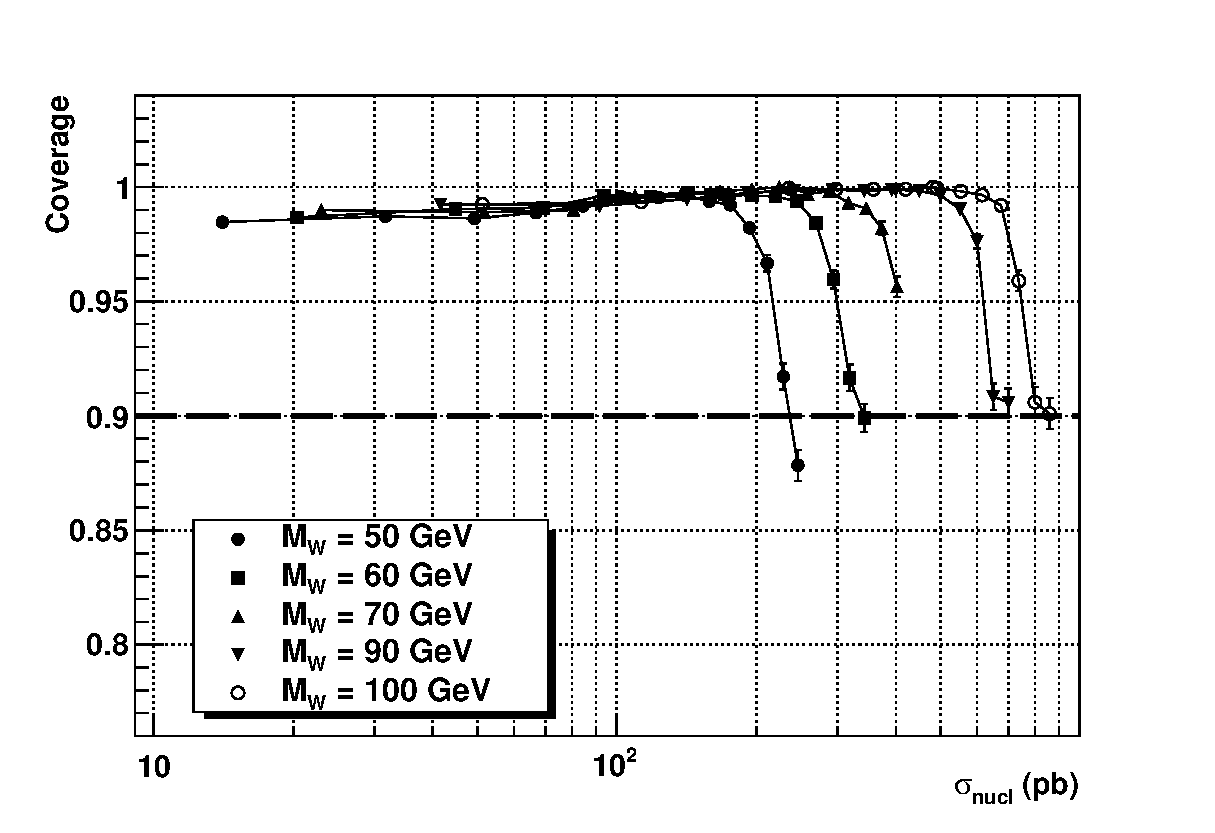
\includegraphics[width=0.46\textheight]{CoverageWithLastWIMP100}
				\label{fig:Coverage100}						
			}	
			% FixME JFW, why the different x axis ranges?				
			\caption[Coverage test results for WIMP mass range 4.25$\to$100~GeV]
			{Coverage test results for WIMP mass range 4.25$\to$100~GeV, see text for details. The range of the x axes ($\signuc$) differs since the coverage scans only
			cover values of the profile likelihood that satisfy $\pll \leq 2$.}
			\label{fig:CoverageTestResults}
		\end{sidewaysfigure}

Rolke et al.~emphasize that correct application of their method~\cite{Rol05} must be accompanied by a coverage test analyzing its effectiveness.  The protocol for this test is outlined in Section~\ref{sec:LimitsUnknownBackgroundML} where it is made clear that the \emph{entire} range of possible parameter space must be scanned.  For all but the most simple models, this is essentially impossible and so it is necessary to reduce the parameter space to a manageable size by selecting those parameter combinations which are the most `likely'.  Since we are primarily concerned with the coverage of the model versus the amount of included signal (proportional to $\signuc$), it is reasonable to use $\pll$ to define the considered parameter space.  $\pll$ provides a 1-dimensional path parameterized by $\signuc$ along an extremum in likelihood space, basically allowing the data to define which parameters of the model are the most likely.  It also reduces the scanned space to one dimension\footnote{In practice, the dimension is still 2 taking into account the variation of the WIMP mass.} thereby reducing the numerical problem to something tractable.  
To perform these tests, a model and a set of data were chosen to be the same as used throughout this section: the model used constrained the relative amplitudes of the Ge and Zn L-capture lines (see Section~\ref{sec:LimitsConstrained}) and the data used was that with a 99\% rise-time cut applied.  Each fit during this procedure was unbinned.  For each WIMP mass, a profile-likelihood function was calculated for $\signuc$ by calculating the maximum likelihood along a grid in $\signuc$-space.  At each point on this grid, the results of the fit (i.e.~parameter values maximizing $L$) were saved for later use.  Points were then selected from the $\pll$, first taking the best-fit result ($\pll = 0$) and then sampling the remainder of the space $\signuc > 0$ and $\pll \leq 2$ for 14 more points.  For each of these 15 points, 2400 toy simulations were run\footnote{For WIMP masses 5.5, 11, 70, and 100~GeV only 2000 toy simulations were run.  This was solely due to scheduling issues on the computer cluster used.} generating events according to the distributions defined by the parameters.  Since the models used an extended-likelihood formalism, the number of events generated for each simulation was poisson distributed according to model parameters.  For each simulation, limits were calculated at 90\% confidence level using the Rolke technique.  The $\sim1$M simulations took roughly 1~year of 2.5~GHz CPU clock time, running on the Athena cluster at the University of Washington~\cite{Athena}.  

Results of these simulations are shown in Figure~\ref{fig:CoverageTestResults}, where the coverage is defined as the percentage of time the calculated limits included the `true' parameter value of $\signuc$, the value used to simulate the data se.  The results from the range of WIMP masses are split into four different plots and grouped together according to similar mass.  Each plot includes a line at 0.9, designating the expected coverage percentage as defined by the input confidence level.  These results indicate in general good coverage with under- and over-coverage mostly limited to within 5\% of the expected value.  The significant over-coverage for larger WIMP mass suggests that over the lower range values of $\signuc$, the signal is completely indistinguishable from background.  The coverage does tend back to 90\% at larger values of $\signuc$.  The under-coverage in Figure~\ref{fig:Coverage13} is likely due to the similarity of exponential background and WIMP signal and could also be affected by the profile-likelihood features discussed in Section~\ref{sec:LLPathologies}.  It is encouraging, however, that despite the fit difficulties and likelihood features discussed in Section~\ref{sec:LLPathologies}, the coverage remains close to 90\%.  This suggests that the Rolke method as applied to this model and data set is robust and that exclusions determined at 90\% confidence level are valid.

		\subsection{Limits from unbinned and binned ML fits.}
		\label{sec:LimitsUnbinned}

Limits were calculated using data described in Chapter~\ref{chap:AnalysisBeGe} and the model in Section~\ref{sec:LimitsDataAndModel}.  The RooFit framework includes an abstracted interface for all data sets, making a transition between using a binned and unbinned analysis very simple and enabling a comparison between the two types of results.  Therefore, both binned and unbinned limits were calculated, selecting a bin size of 23.4~eV over the energy range (0.5$\to$3.5~keV, bin number: 128).  
Fits were performed for chosen values of $M_{W}$ in the range $3.75\to100$~GeV, sampling different ranges of the mass with a variable step size, $\Delta$: $3.75\to11$, $\Delta=0.25$~GeV; $11\to25$, $\Delta=1$~GeV, $30\to100$, $\Delta=10$~GeV.  Given the large amount of fits required to generate, the calculation method was parallelized for submission to the Athena cluster~\cite{Athena} at the University of Washington.  
			\subsubsection{Fit components versus \texorpdfstring{$\signuc$}{sigma\_nuc}}
When running a large number of fits, it is challenging to provide effective quality control to ensure that the limit calculation has proceeded correctly.  To check this, the parameters of the values were tracked at their best-fit value (defined as the minimum $-\log L$ in the region $\signuc\geq0$) and at the 90\% exclusion limit of $\signuc$.  Examples of two of these plots are given in Figures~\ref{fig:UnbinnedResultsNoConstrain} and~\ref{fig:BinnedResultsNoConstrain} which are for unbinned and binned results, respectively.  The top three plots in each of these figures includes the individual components of the background events: the counts-per-kilogram-per-day in the exponential, flat, and separate L-line backgrounds.  The bottom plot includes the sum of the flat and exponential background and the sum of the Ge and Zn L-capture lines.  The parameters are generally smoothly varying versus $\signuc$ except in the region $\sim6\to10$~GeV where a significant amount of oscillation can be seen in the amplitudes of the flat and exponential components.  This oscillation is due mainly to the fact that the exponential shape constant is allowed to float positive and therefore can become indistinguishable from the flat background.  This is also confirmed by the largely-smooth behavior of the sum of the exponential and flat background components.  An example of the variation of the exponential shape parameter is discussed in Section~\ref{sec:LLPathologies} and shown in Figure~\ref{fig:FitExpoShapeVsSigma}.  However, some large variations do remain in the best-fit values of the sum components; these are due to the appearance in this WIMP mass region of local extrema away from the global minimum (see Figure~\ref{fig:PLLRangeSeven}).  Since the global extremum may be in the disallowed region (i.e.~$\signuc<0$), it is possible that the local minima are then interpreted as the global minima (i.e.~the best fit), but this is dependent on the granularity of the scanned $\signuc$ space and the size of the local minimum since it is possible to not sample fully the local minimum if it has a small width.  In other words, it is possible to `skip over' the local minimum and therefore interpret $\signuc=0$ as the best fit.  However, despite the sharp features in the best-fit values of the exponential and flat components it is clear that the value of the sum of these components at the 90\% exclusion of $\signuc$ varies smoothly.  

The amplitudes of each L-line component vary quite little versus $\signuc$.  Additionally, there is little to no difference between the amplitudes of these components at the global minimum and at the 90\% exclusion of $\signuc$.  This indicates that this portion of the background has little effect on the calculation of limits on a WIMP signal.

All of the same conclusions may be drawn from the binned analysis of the same data, results of which are shown in Figure~\ref{fig:BinnedResultsNoConstrain}.  As with the unbinned data, it is clear that some sharp features exist in the best fit of the sum of the flat and exponential components.  Regardless, the smoothness of the sum of the parameters at the 90\% exclusion of $\signuc$ implies that any sharp variation in the best-fit parameters are irrelevant.  The similarity between binned and un-binned results indicates the robustness of the maximum-likelihood technique and also suggests that an unbinned analysis could be unnecessary for data with this number of counts.
  
			\begin{figure}
				\centering				
				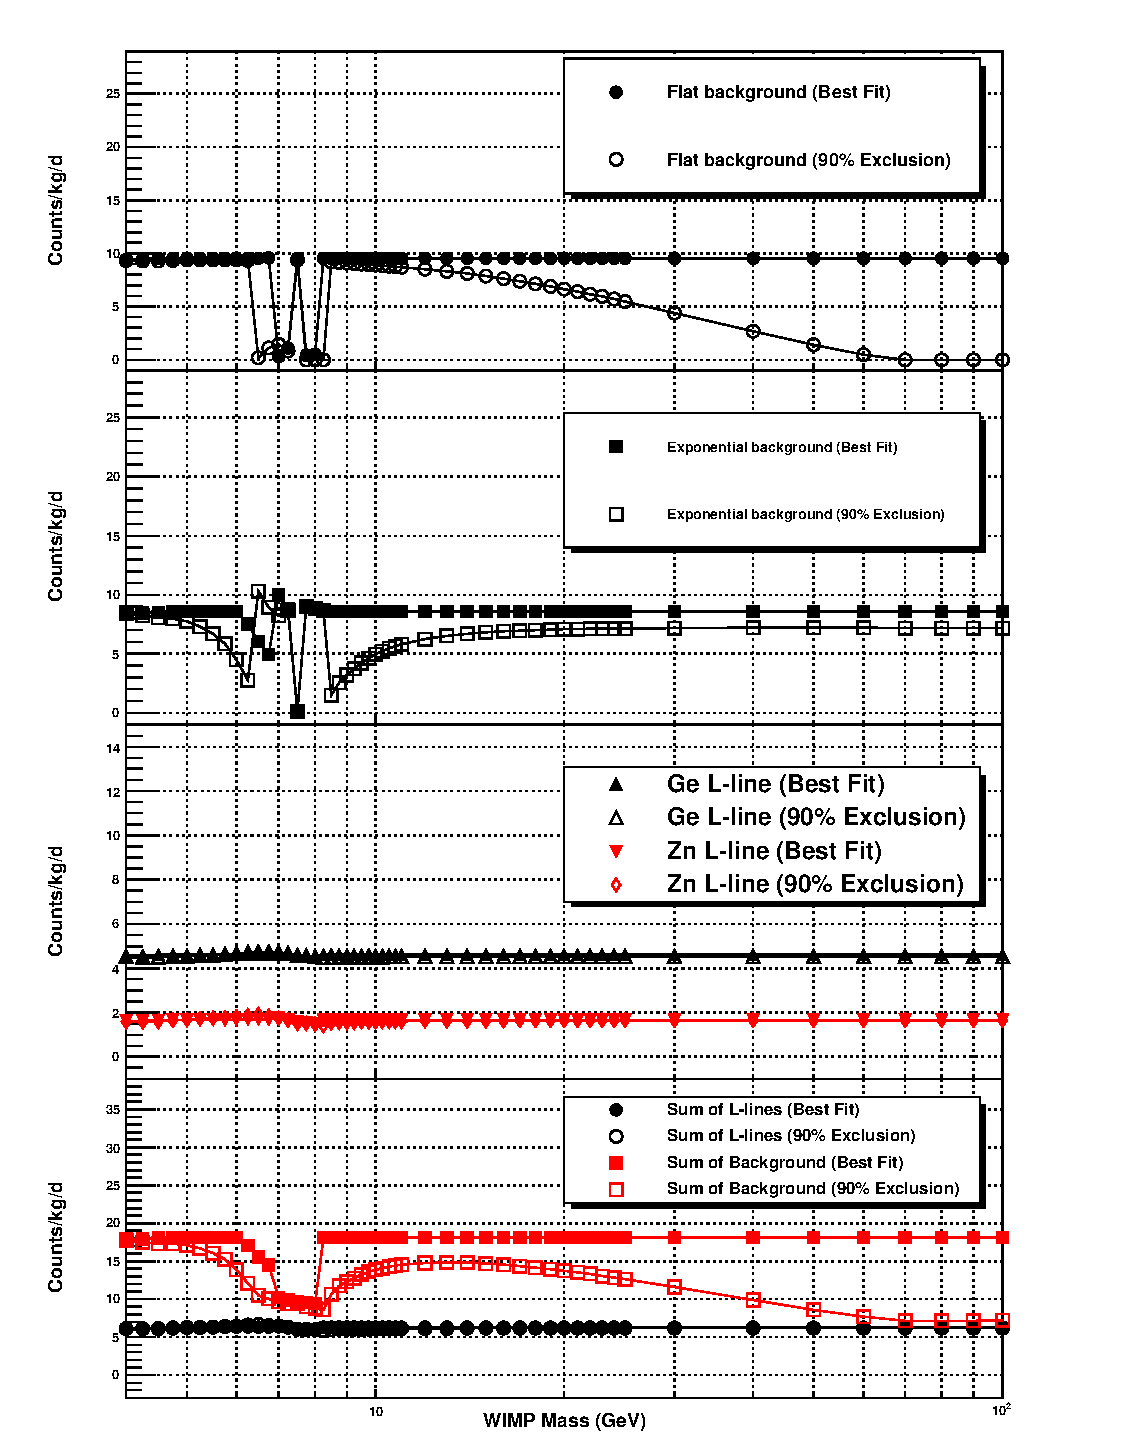
\includegraphics[width=0.85\textwidth]{unconstrained_unbinnedresults_rt_95AllComponentsLN+microphonicscuts,Rise-timecut:95}				
				
				\caption[Fit results using unbinned data with 95\% risetime cut (+ microphonics cut) applied]
				{Results from an unbinned fit using data with 95\% risetime cut (+ microphonics cut) applied.
				The top three figures contain the variation of all independent parameters at their best-fit value and at the 90\% exclusion
				limit of $\signuc$.  The bottom figure contains a sum of the background components (flat + exponential) and
				the L-lines.  See text for details.  Lines between points are included to guide the eye.}
				\label{fig:UnbinnedResultsNoConstrain}
			\end{figure}
			\begin{figure}
				\centering				
				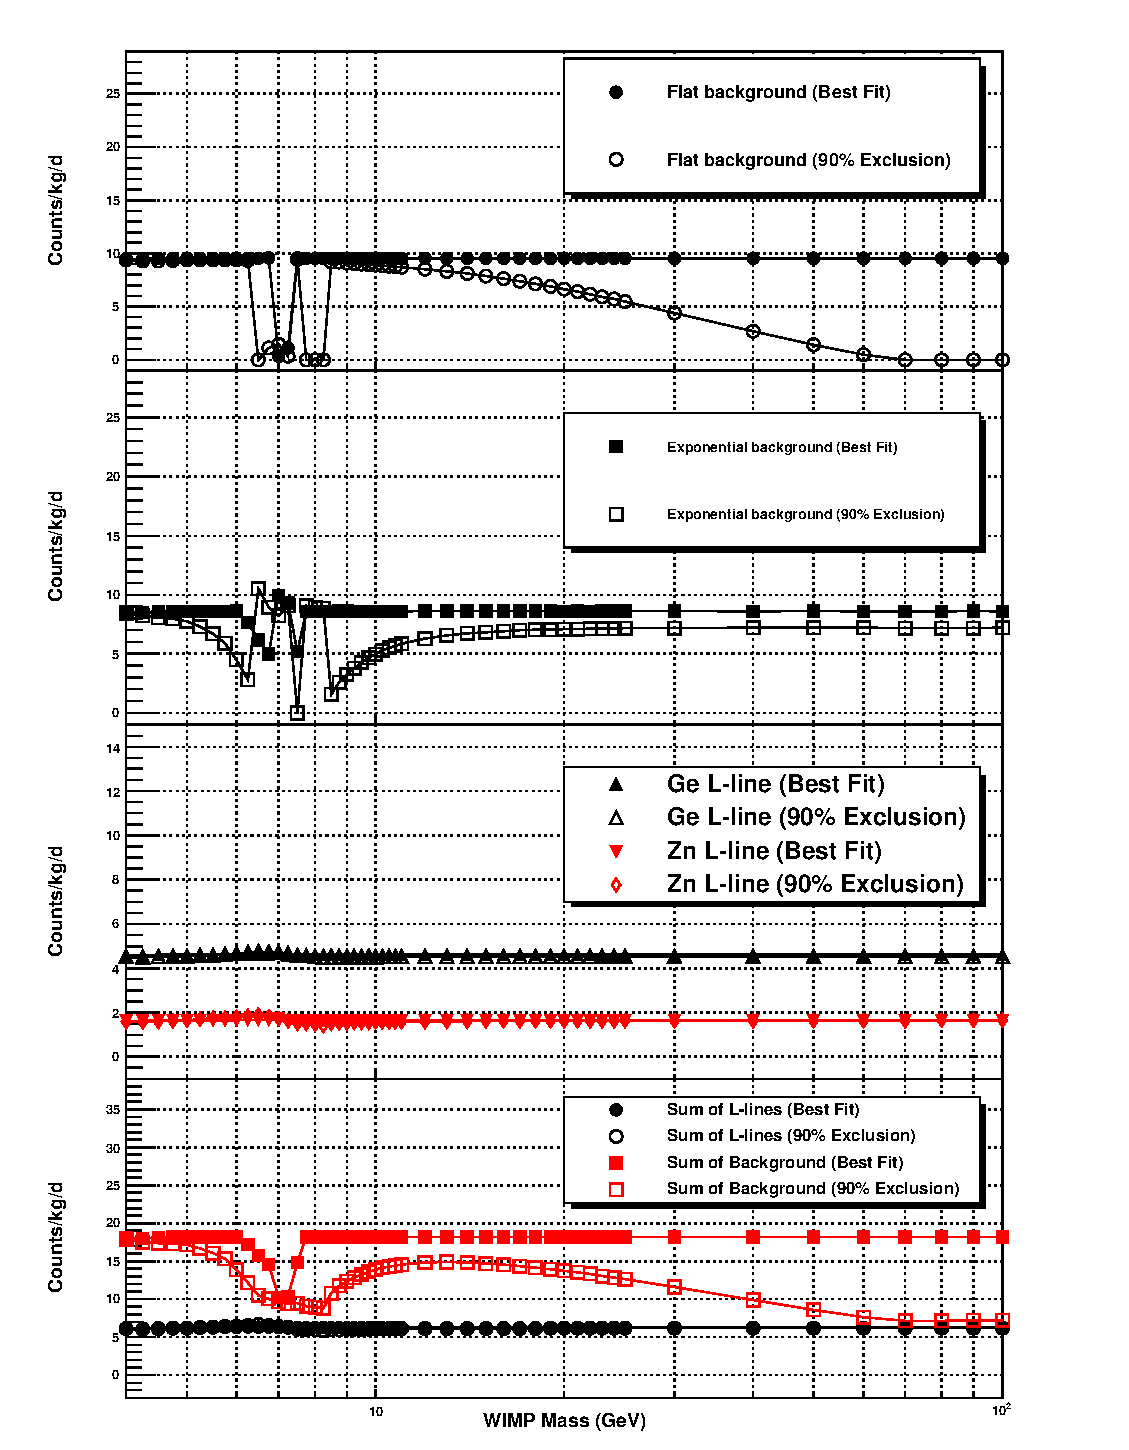
\includegraphics[width=0.95\textwidth]{unconstrained_binnedresults_rt_95AllComponentsLN+microphonicscuts,Rise-timecut:95}				
				
				\caption[Fit results using binned data with 95\% risetime cut (+ microphonics cut) applied]
				{As Figure~\ref{fig:UnbinnedResultsNoConstrain} but with binned data.}
				\label{fig:BinnedResultsNoConstrain}
			\end{figure}
			
			\begin{sidewaysfigure}
				\centering
				\subfigure[Unbinned]{
					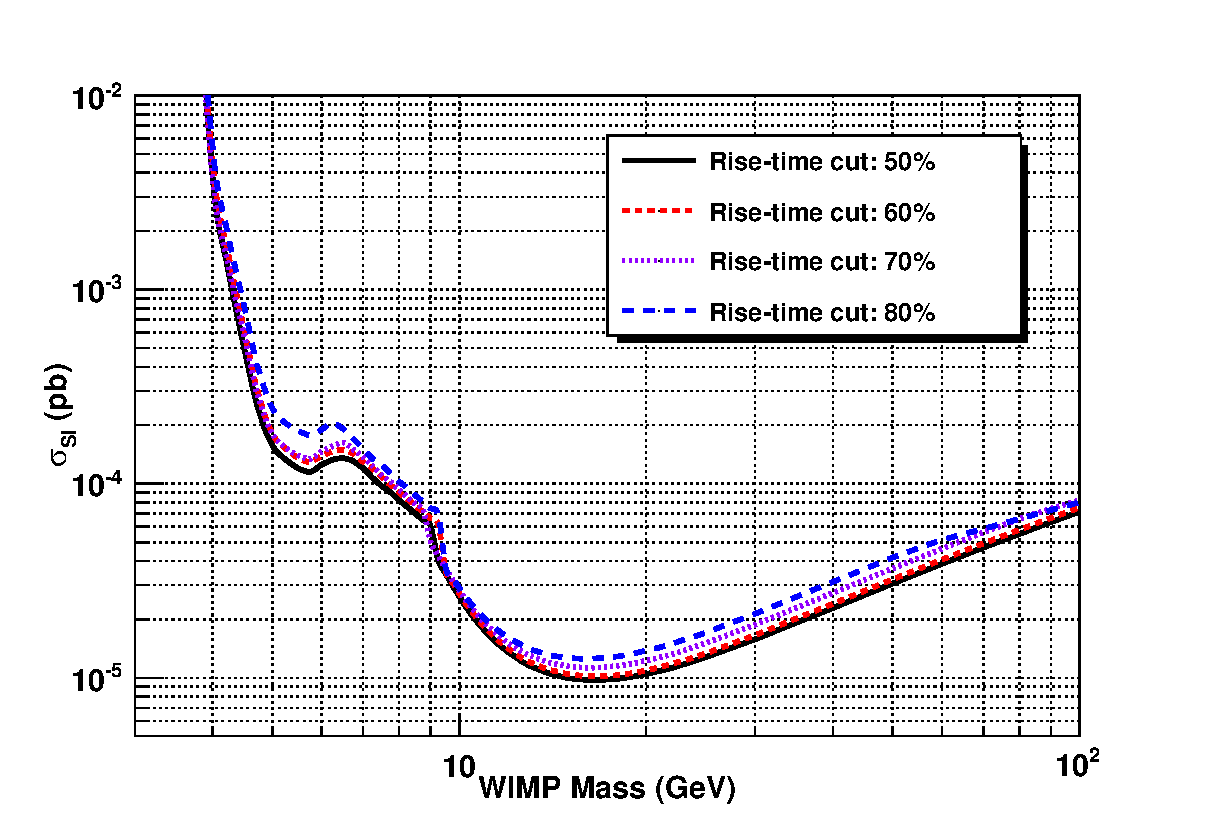
\includegraphics[width=0.46\textheight]{unconstrained_unbinnedall_exclusion_plots80}
					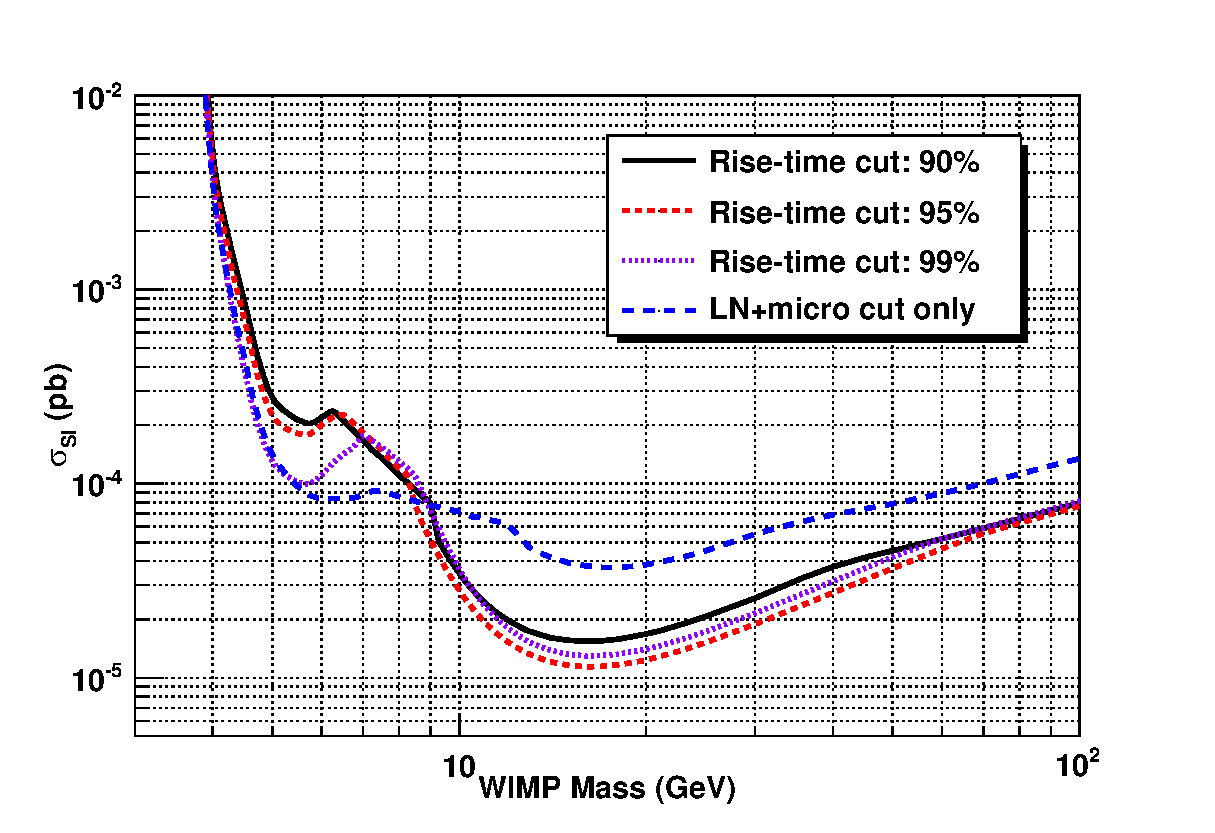
\includegraphics[width=0.46\textheight]{unconstrained_unbinnedall_exclusion_p1000}
					\label{fig:UnconstrainedLimitsUnbinned}						
					
				}												
				\subfigure[Binned]{
					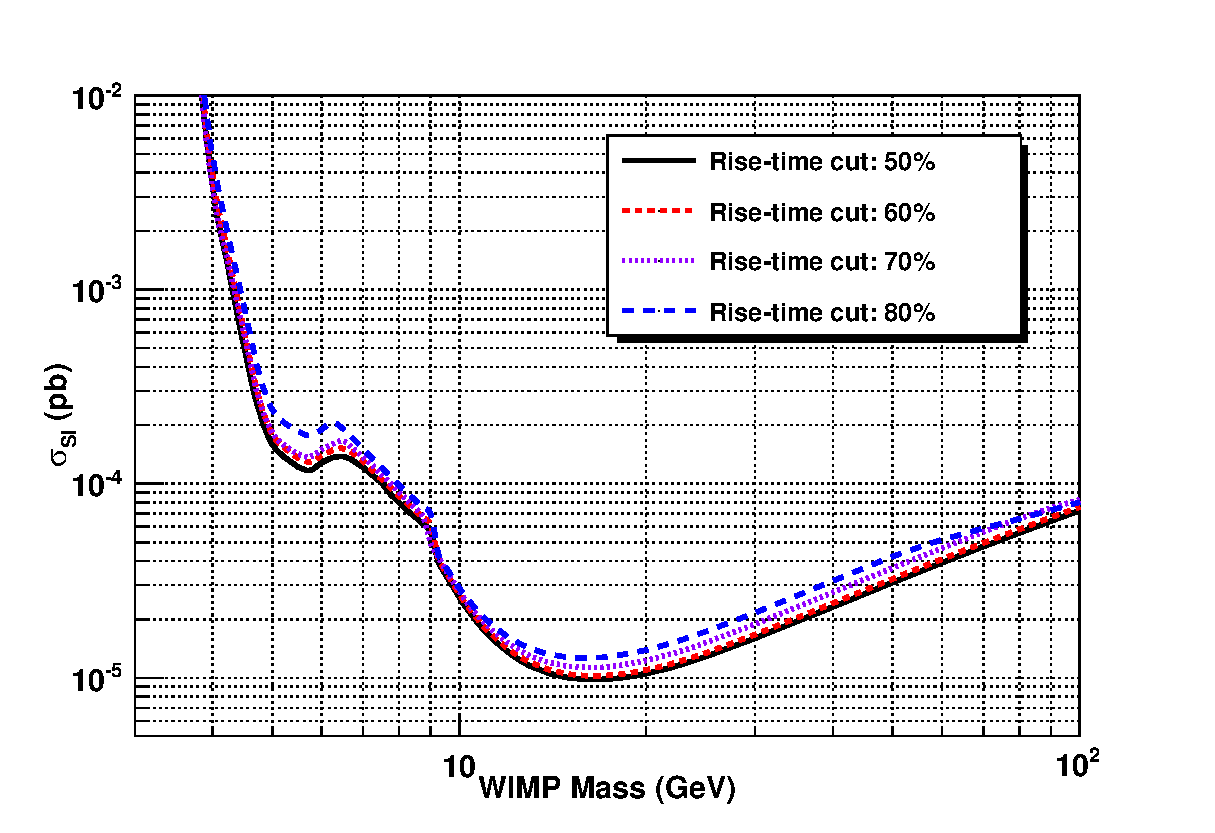
\includegraphics[width=0.46\textheight]{unconstrained_binnedall_exclusion_plots80}
					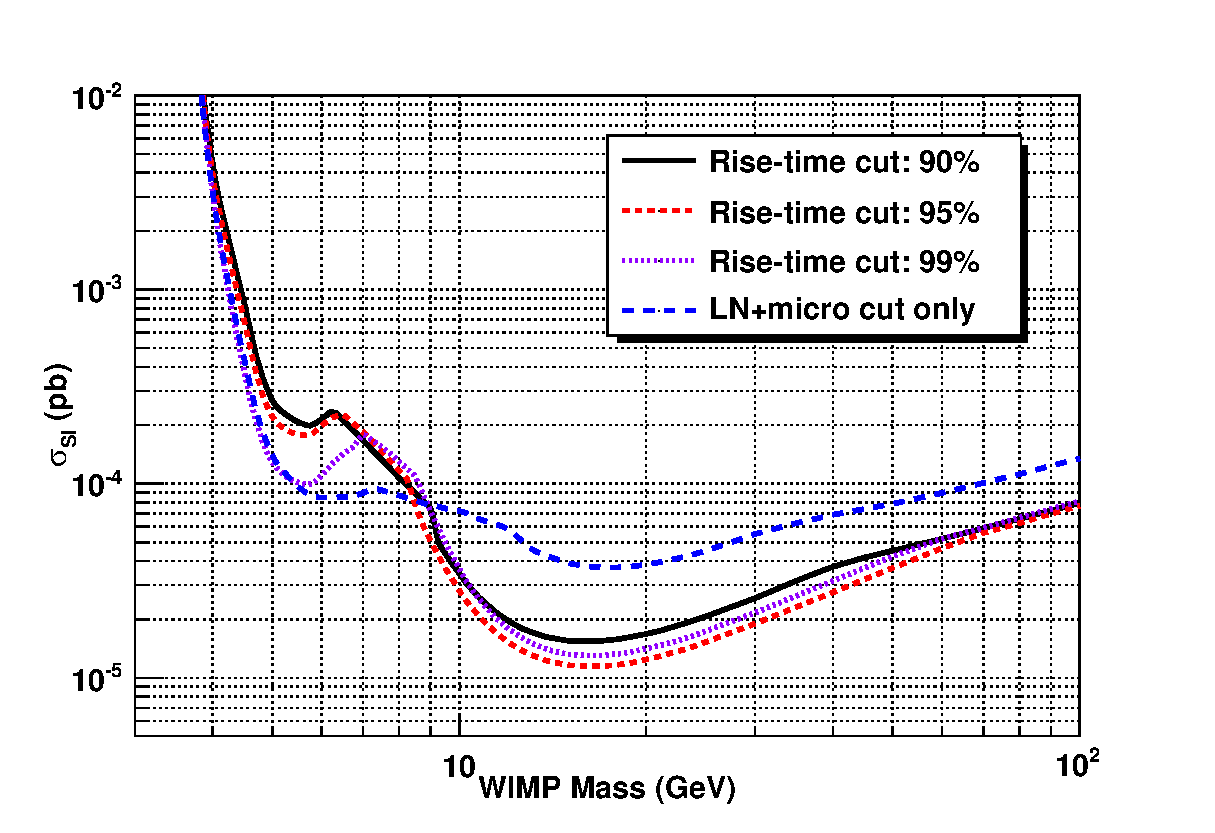
\includegraphics[width=0.46\textheight]{unconstrained_binnedall_exclusion_p1000}				
					\label{fig:UnconstrainedLimitsBinned}						
				}
				\caption[90\% CL limits on $\sigman$ for various data sets]
				{90\% CL limits on $\sigman$ for various data sets.}
				\label{fig:UnconstrainedLimits}
			\end{sidewaysfigure}			
			
			\subsubsection{Exclusion limits}	
Exclusion limits at 90\% confidence level for $\sigman$ are shown in Figure~\ref{fig:UnconstrainedLimits}, with $\sigman$ calculated from $\signuc$ given the relationship in Equation~\ref{eqn:SigmaConversion}.  Results for both binned and unbinned data are split into two plots each to allow clearer visualization of exclusions calculated for data sets with different cuts applied.  
It is clear that there exists very little distinction between limits on binned and unbinned data; however, several features are apparent among the different data sets.  In the low-WIMP-mass range, 4-5.5~GeV, all the curves are very similar suggesting the limits in this small region are robust against cuts to the data.  At higher WIMP mass, 20-100~GeV, the slope of the curves is very similar, though the normalizations are somewhat different.  As expected, in this region the microphonics-cut data exhibits more conservative limits than the rise-time cut-data.  The variation in the limits calculated from rise-time-cut data is expected to arise from systematic errors on the estimation of the efficiencies of these cuts as well as from the unknown ratio, (signal)/(signal + background), for each cut.  

The mass range 6-9~GeV exhibits sharp features in the exclusion plots, existing in WIMP-mass regions where the shape of the signal is very similar to the shape of the background.  These features also appear in the microphonics-cut data, but at a slightly higher mass range from $\sim7\to10.5$~GeV.  These characteristics are essentially an indication that the calculated exclusion limit comes when the amplitude of the WIMP signal completely takes over the contribution from the exponential fit component.  An example of this is given in Figure~\ref{fig:WIMPFitExampleSigLikeBgd} which displays the fit at the 90\% CL exclusion of $\sigman$.  It is clear that at this value of $\sigman$, the WIMP signal fits to the low-energy data without any contribution from the exponential background.  Close inspection also reveals that the exponential shape parameter has transitioned to a positive value, resulting in a mildly increasing background with energy.  

			\begin{figure}
				\centering
				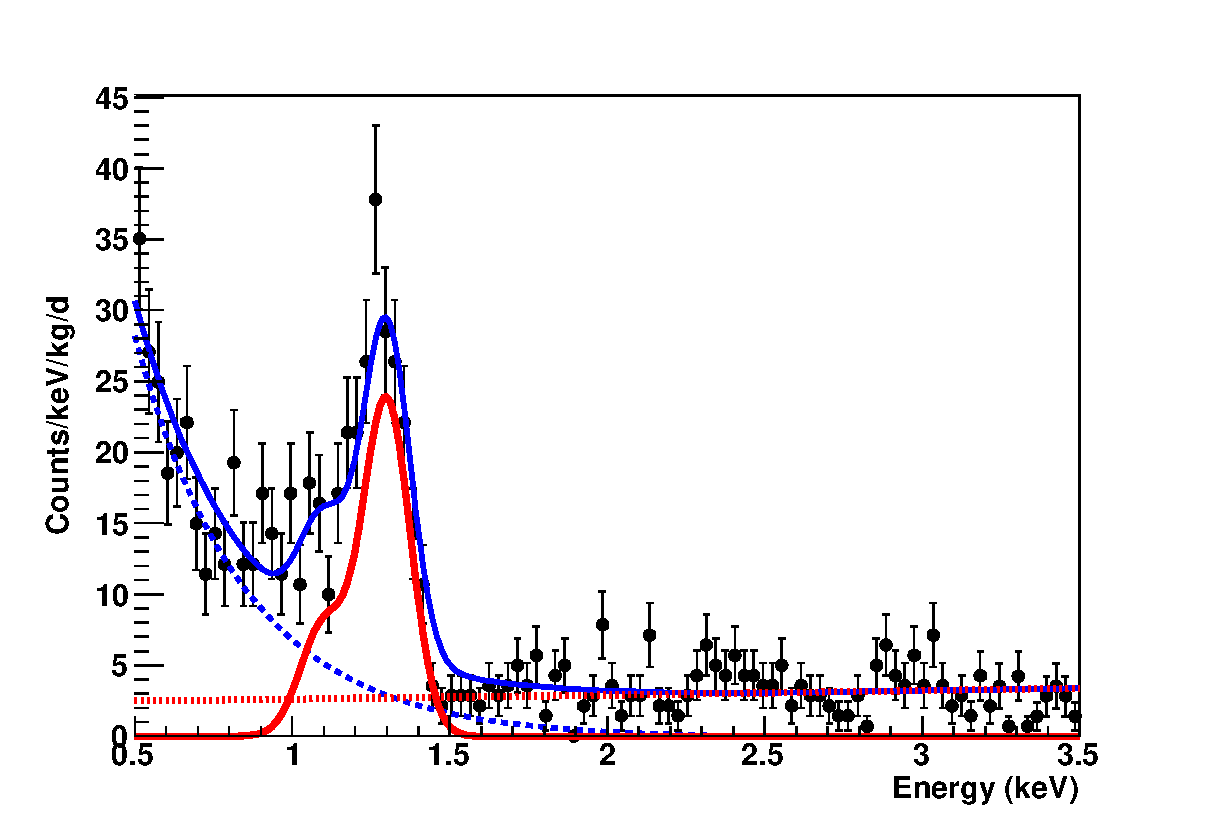
\includegraphics[width=0.9\textwidth]{WIMPMass8GeVFinalFit}
				\caption[Signal exclusion fit at 90\% CL.]
				{Fit at 90\% CL exclusion, $\sigman = 1.2 \times 10^{-4}$~pb.  
				WIMP signal is blue dashed, L-lines in solid red, flat + exponential background in dotted red, and 
				sum of all the pdfs is blue solid.
				This is an unbinned fit with 95\% rise-time cut data.  }
				\label{fig:WIMPFitExampleSigLikeBgd}
			\end{figure}

At low-mass range the microphonics-cut data demonstrates a stronger limit than the 80\%$\to$99\% rise-time-cut data.  Initially this seems counter-intuitive, but can be explained due to the fact that the microphonics-cut data includes a larger contamination of slow-rise-time pulses which is not well fit with a single exponential.  This indicates that the background distribution coming from slow rise-time pulses is not properly included in the set of background pdfs.  Since this distribution is not known a-priori, the proper inclusion would require a source measurement to estimate its shape.  It is interesting to note that the exclusion calculated using 99\% rise-time cut data demonstrates a transition between the microphonics cut data and the 95\% rise-time cut data around 6~GeV.  The shape and coverage of the rest of the rise-time cut exclusions are similar, suggesting that the rise-time cut retains a consistent shape in the data as the acceptance is decreased from 99\%.  It also implies that some slow-rise-time-pulse background remains at 99\% acceptance, consistent with results from Section~\ref{sec:RisetimeSystematicTests} which demonstrated a slightly less-negative exponential constant with the 99\% rise-time-cut data as compared to rise-time cuts with less acceptance.  This final conclusion indicates that data with at least a 95\% rise-time cut should be used to generate exclusions since these data will have as little slow-rise-time-pulse contamination as possible.  

		\subsection{Constrained Ge and Zn relative amplitudes}
		\label{sec:LimitsConstrained}
	
The relative amplitudes of the Zn and Ge L-capture lines may be constrained by the K-capture lines of the same isotopes since the K- to L-capture ratio has been well understood through independent measurements~\cite{Bea67,Ocampo1962}, see Table~\ref{tab:LKRatios}.  The amplitudes (in counts) of the Ge and Zn K-lines were measured using an unbinned fit of the 99\% rise-time-cut data\footnote{The 2~month live-time data was used to calculate this ratio.} and determined to be 945.125$\pm28.2$ and 349.65$\pm19.1$, respectively\footnote{This measurement was performed using a smaller subset of data with 2~months of live-time.}.  Therefore, the expected ratio of the Ge and Zn lines (Zn/Ge) was 0.33$\pm$0.03.  The relative amplitudes of these lines in the fitting model were then constrained by this value, reducing the number of parameters in the fit by one.  In general, it would be more desirable to tie this ratio to the amplitudes of the K-capture lines and perform a simultaneous fit, but since the relative amplitudes of the lines did not vary significantly when allowed to float independently and since the measurements of each set of lines were in separate channels (high-, low-gain channels for L-,K-lines, respectively), it was not expected that proceeding in such a manner should have a significant impact.  Final results of the fit supported this initial assumption.
	
			\begin{table}
				\centering
				\begin{tabular}{lcr}
					\toprule
					Atom & Value & Ref.\\
					\midrule
					Ge & 0.1328$\pm$0.002 & \cite{Bea67}\\
					Zn & 0.12$\pm$0.07 & \cite{Ocampo1962}\\
					\bottomrule
				\end{tabular}	
				\caption[L/K capture ratios for Ge and Zn]
				{L/K capture ratios for Ge and Zn.}
				\label{tab:LKRatios}
			\end{table}
			
			\begin{figure}
				\centering				
				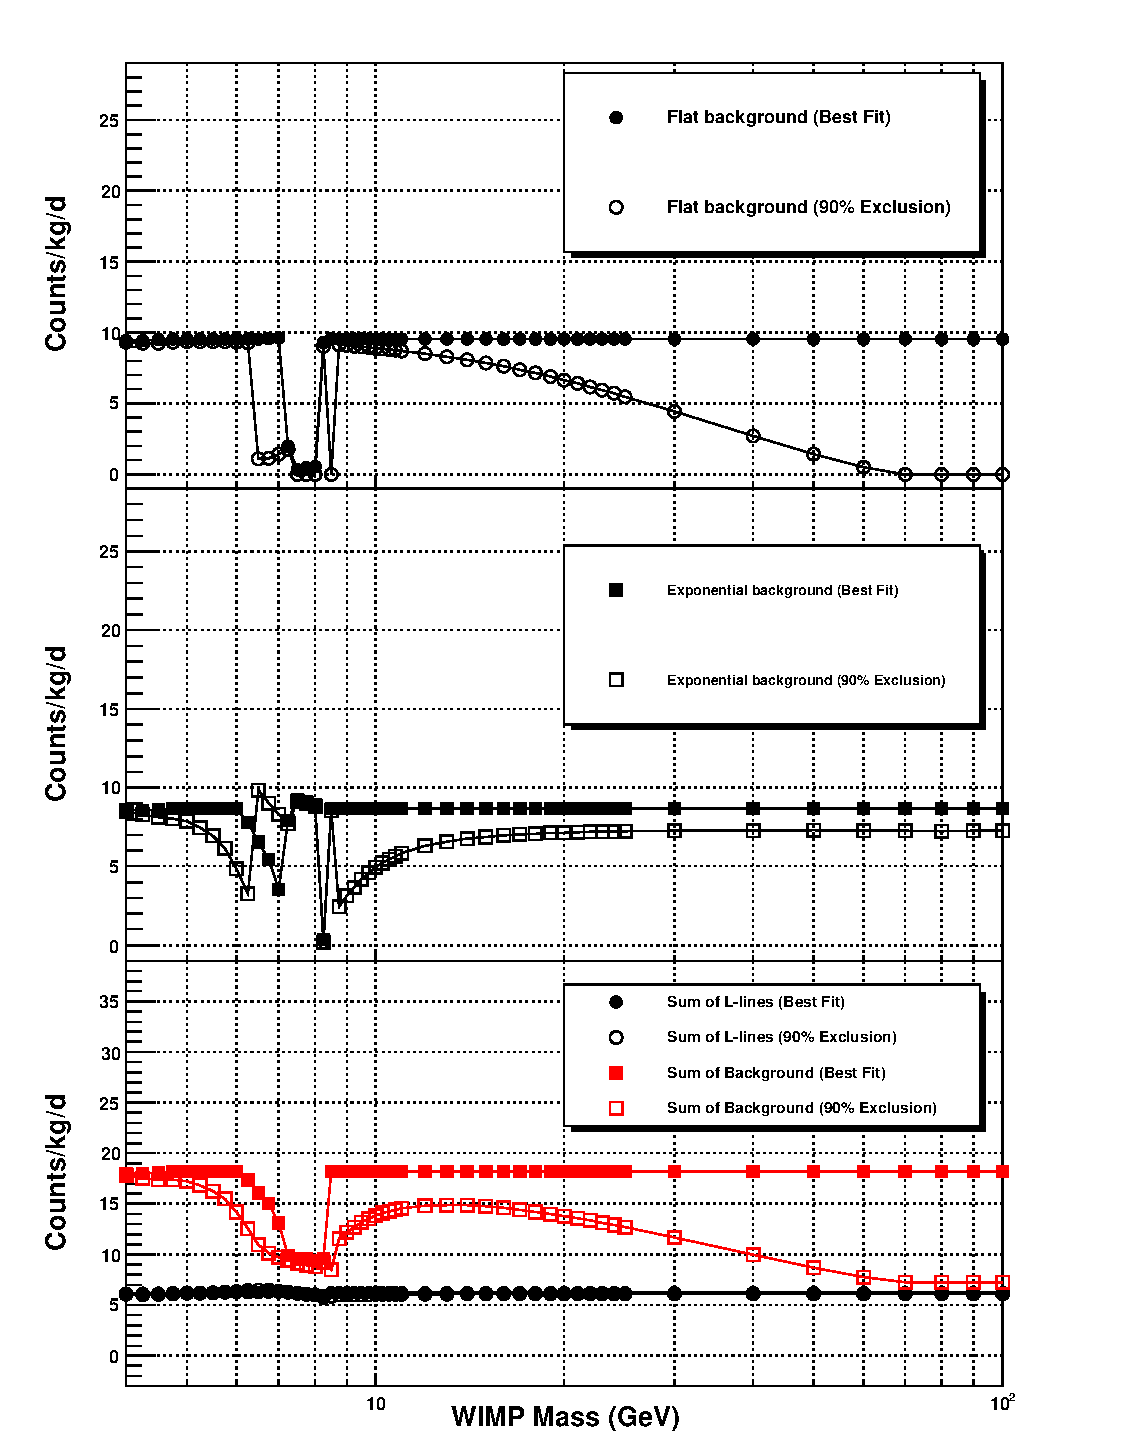
\includegraphics[width=0.95\textwidth]{constrained_unbinnedresults_rt_95AllComponentsLN+microphonicscuts,Rise-timecut:95}				
				\caption[Unbinned fit results, constraints on relative amplitude of Ge and Zn lines]
				{As Figure~\ref{fig:UnbinnedResultsNoConstrain}, but with a constraint on the relative amplitudes 
				of the Ge and Zn lines.  Therefore, only the sum of the L-lines (and not each contribution) is included.  }
				\label{fig:UnBinnedResultsConstrain}
			\end{figure}
					
			\begin{figure}
				\centering				
				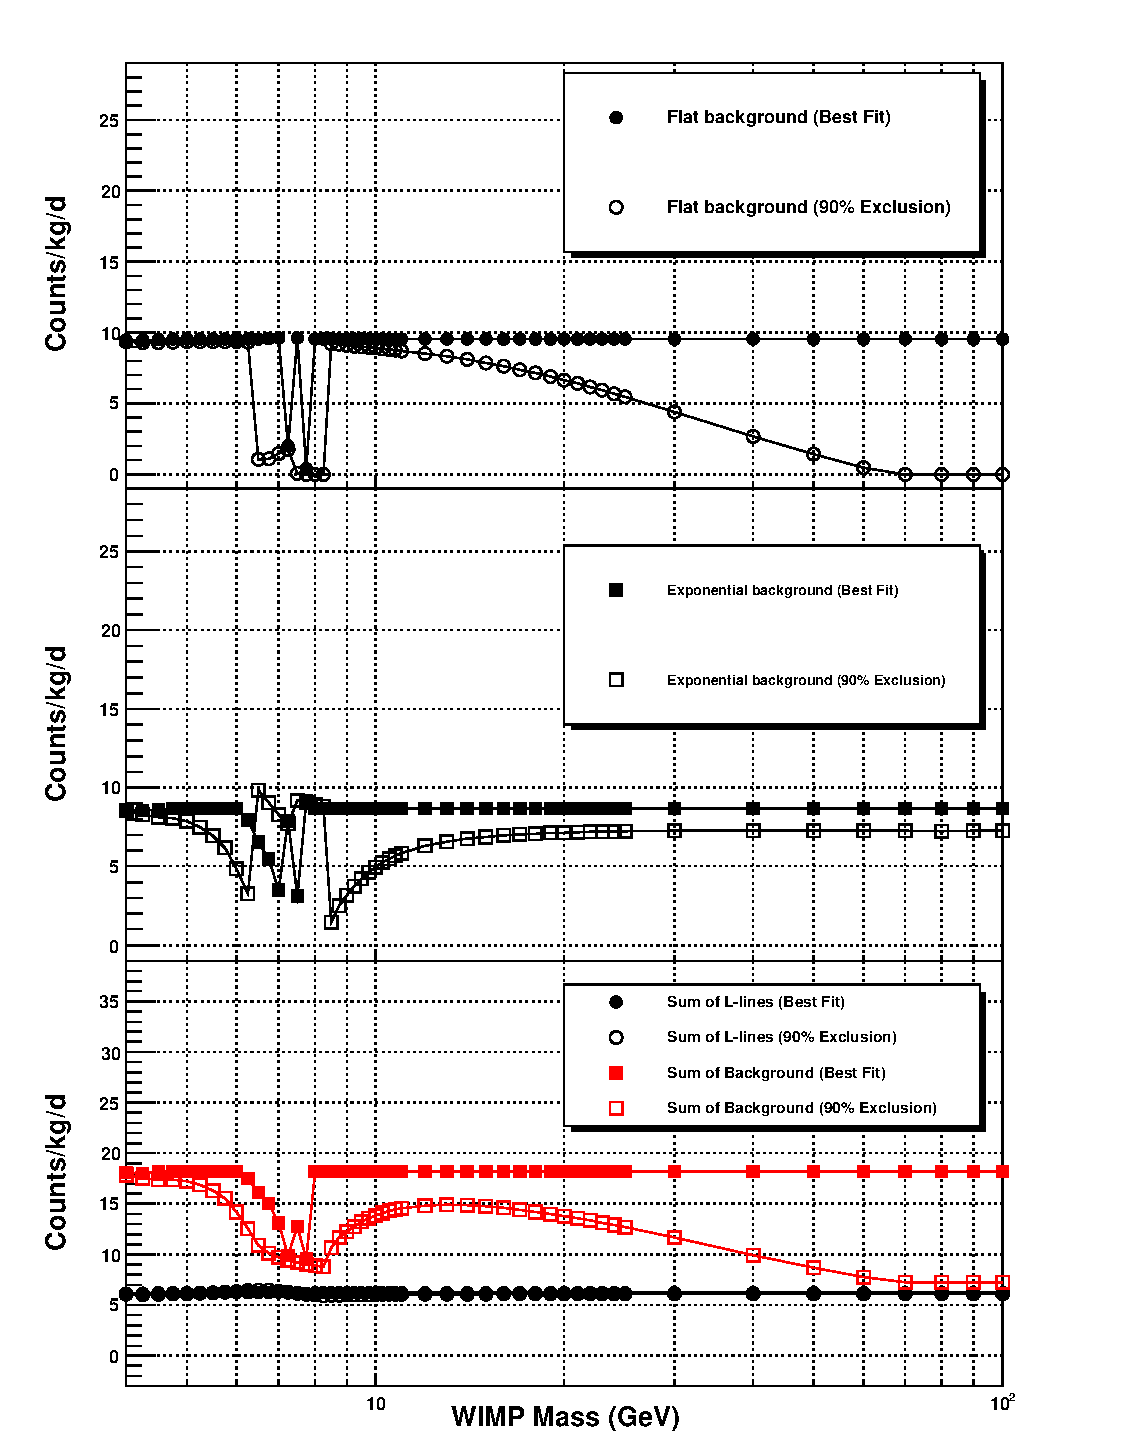
\includegraphics[width=0.95\textwidth]{constrained_binnedresults_rt_95AllComponentsLN+microphonicscuts,Rise-timecut:95}
								
				\caption[Binned fit results, constraints on relative amplitude of Ge and Zn lines]
				{As Figure~\ref{fig:UnBinnedResultsConstrain}, but with binned data.}
				\label{fig:BinnedResultsConstrain}
			\end{figure}
			
			\begin{sidewaysfigure}
				\centering
				\subfigure[Unbinned]{
					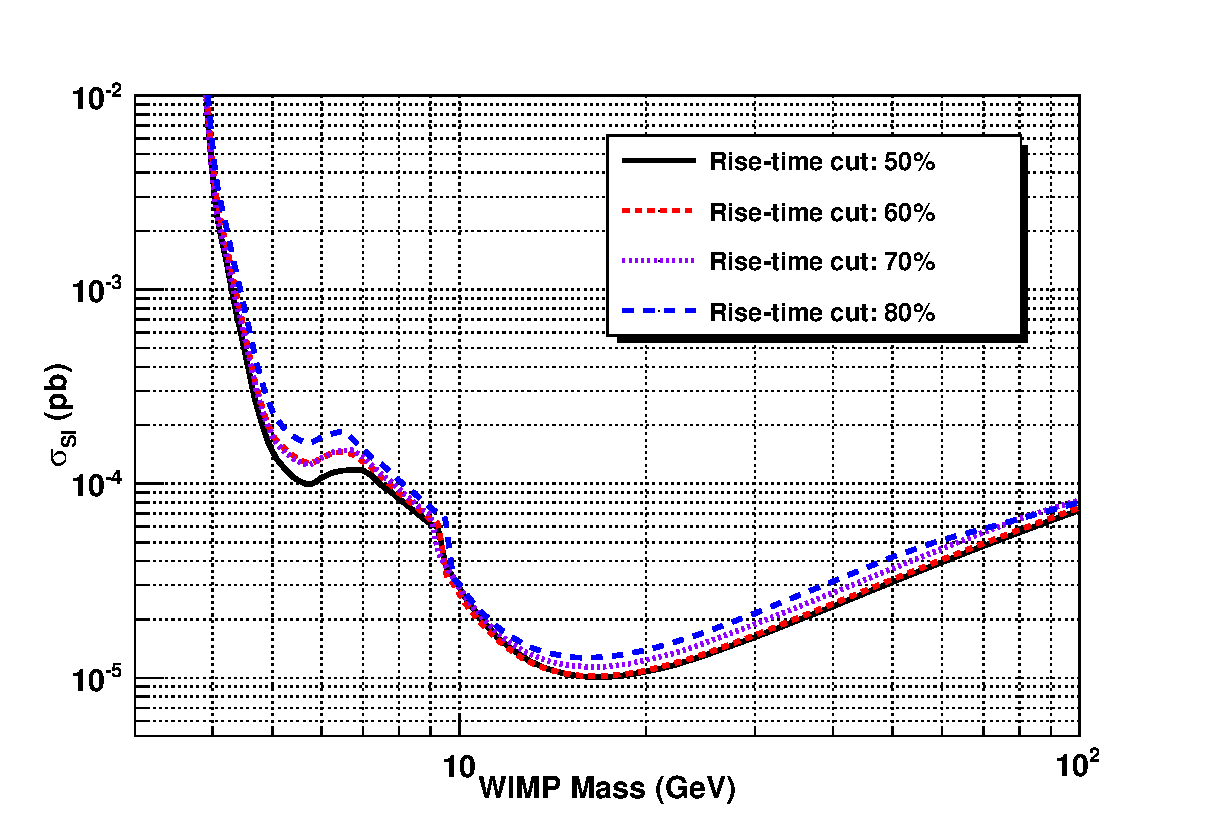
\includegraphics[width=0.46\textheight]{constrained_unbinnedall_exclusion_plots80}
					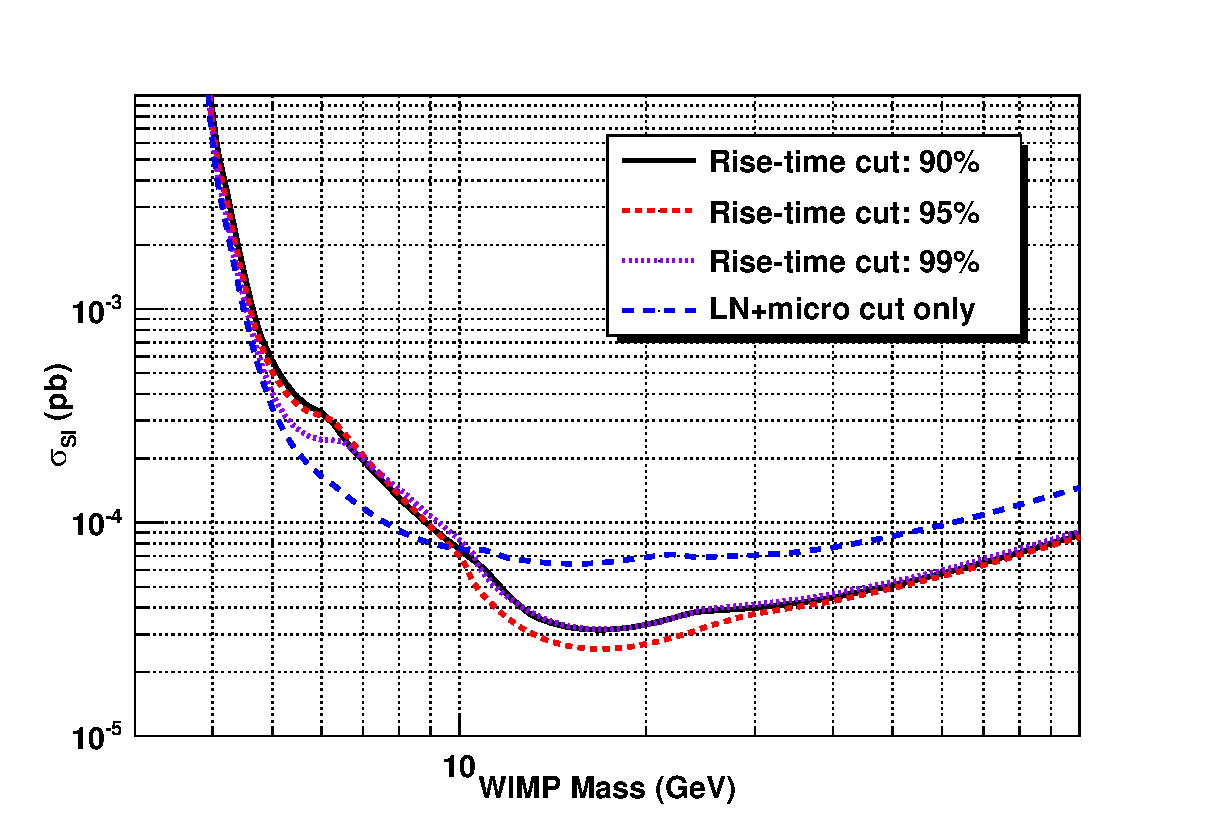
\includegraphics[width=0.46\textheight]{constrained_unbinnedall_exclusion_p1000}			
					\label{fig:ConstrainedLimitsUnbinned}						
				}												
				\subfigure[Binned]{
					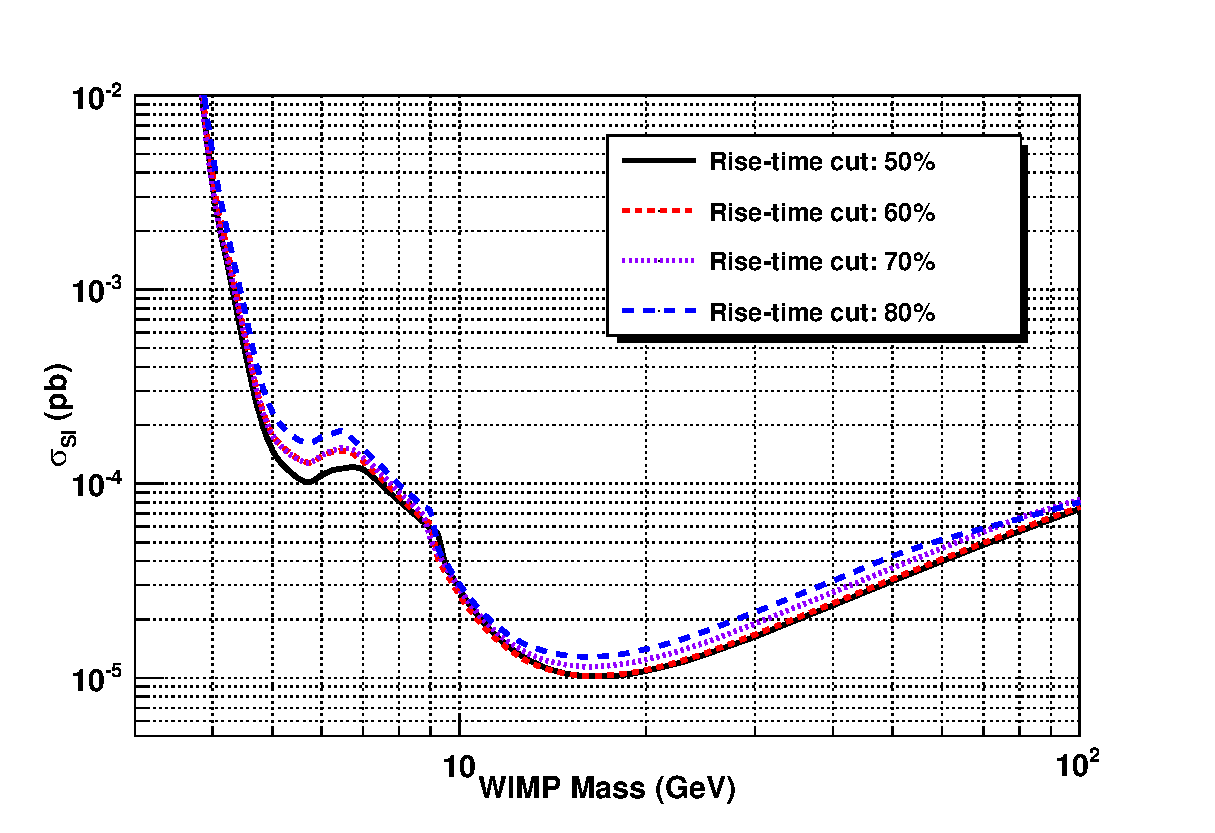
\includegraphics[width=0.46\textheight]{constrained_binnedall_exclusion_plots80}
					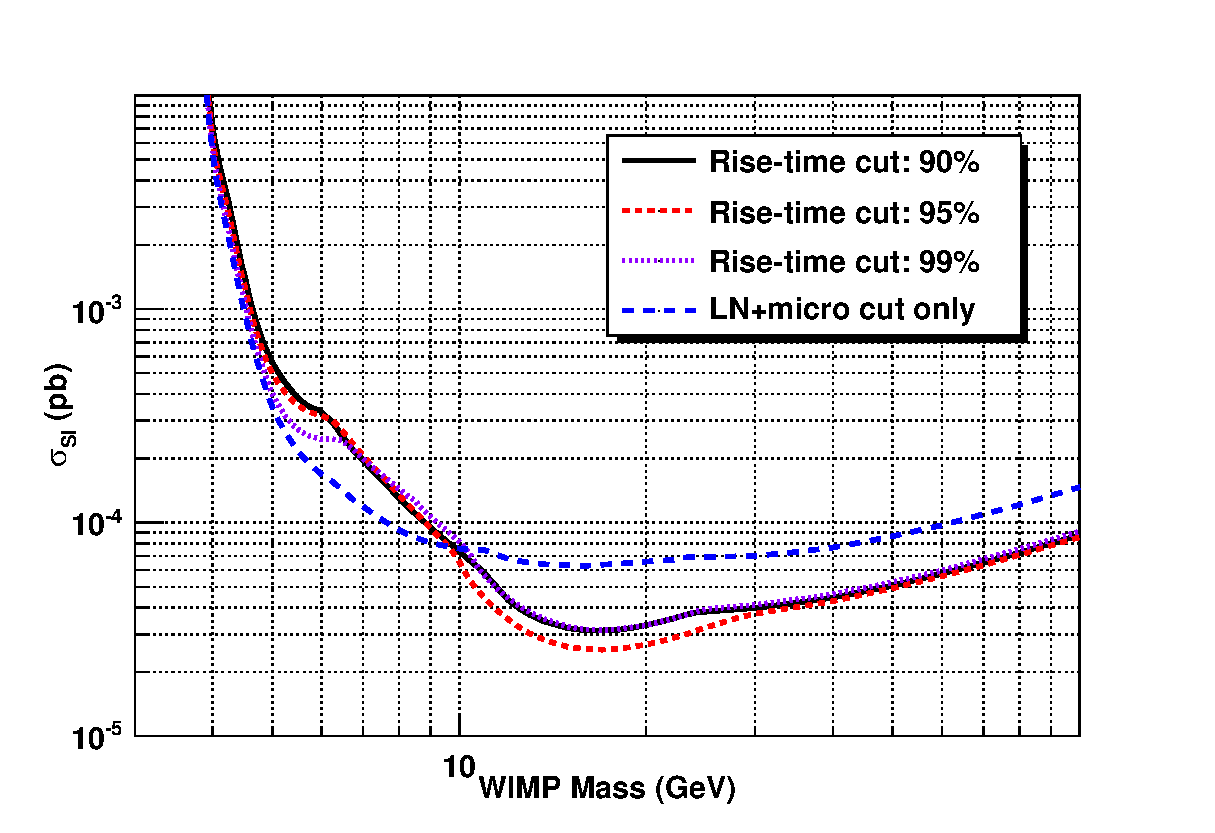
\includegraphics[width=0.46\textheight]{constrained_binnedall_exclusion_p1000}			
					\label{fig:ConstrainedLimitsBinned}						
				}
				\caption[Limits on $\sigman$ constraining the relative amplitudes of Ge and Zn L-lines]
				{Limits on $\sigman$ constraining the relative amplitudes of Ge and Zn L-lines.}
				\label{fig:ConstrainedLimits}
			\end{sidewaysfigure}		
			
Results are presented as in Section~\ref{sec:LimitsUnbinned}, with a representative set of plots of parameters versus WIMP mass (Figures~\ref{fig:UnBinnedResultsConstrain},~\ref{fig:BinnedResultsConstrain}) and exclusion limits in Figure~\ref{fig:ConstrainedLimits}.  As before, it was determined that very few differences manifested between the binned and unbinned results.  The amplitude of the sum of the L-lines appears very similar ($\sim6$~Counts/kg/d) as with the unconstrained fit (Figure~\ref{fig:UnbinnedResultsNoConstrain}).  However, this comes as little surprise given the relative independence and lack of variation of these parameters in the unconstrained fits.  Because of the clear similarity between the constrained and unconstrained results, the conclusions regarding this set are equivalent to the previous.  However, the results of this section further emphasize that the amplitudes of the L-lines have little effect on the exclusion of a low-mass-WIMP signal since the sum of the L-lines varies so minimally with WIMP mass.  Also, little difference exists between the amplitude of the L-line at best fit and at 90\% exclusion, indicating that these parameters have very little sensitivity to $\signuc$.

	\section{Conclusions and discussion}
	\label{sec:LowMassWIMPConclusions}


		\begin{figure}
			\centering
			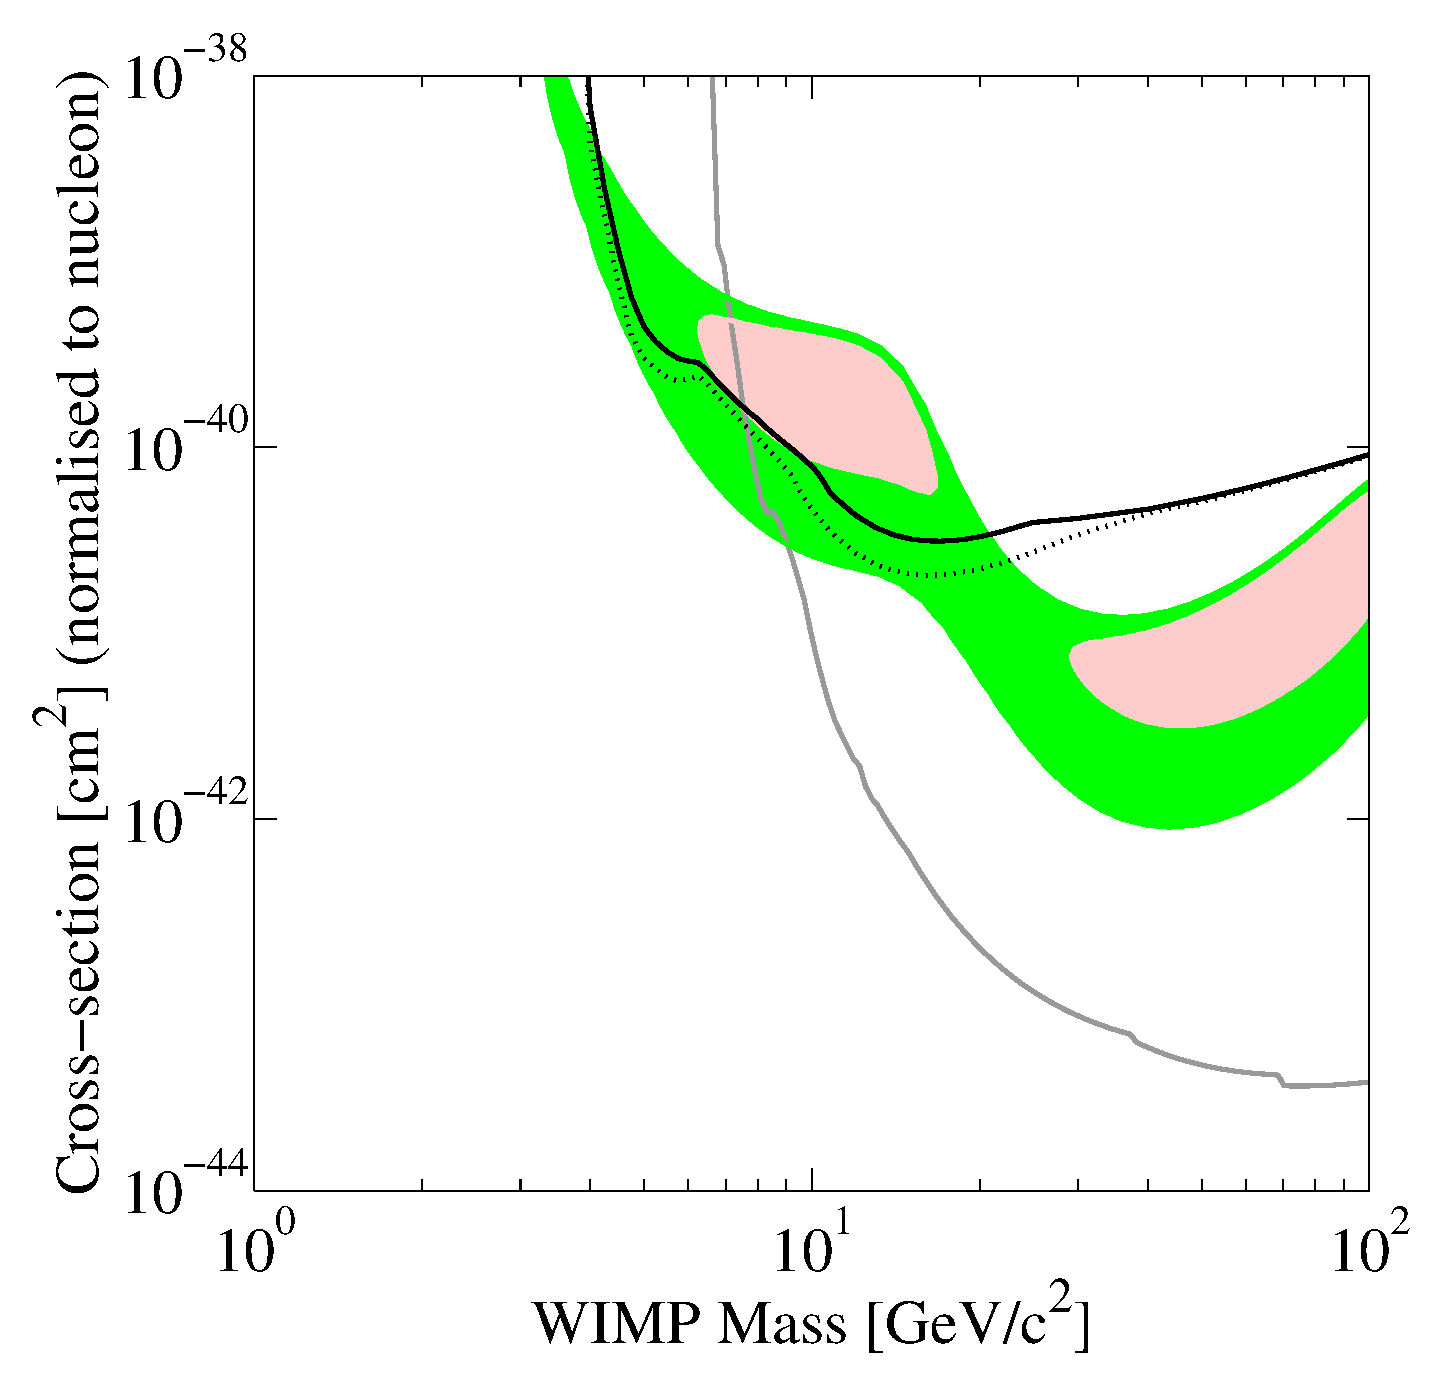
\includegraphics[width=0.9\textwidth]{MGM_Thesis_Compare_plot}
			\caption[Comparison of exclusions to CDMS, DAMA, and previous CoGeNT results.]
			{Comparison of results from this analysis to other results.  Included lines are 90\% CL 
			exclusion limits using 95\% (black dashed) and 70\% (black solid) rise-time-cut data sets, 
			results from the previous CoGeNT detector~\cite{Aalseth:2008aa} (red dotted), 
			most recent CDMS results~\cite{Ahmed:2009zw} (gray solid), and acceptance regions
			from DAMA data as interpreted in~\cite{Savage:2008er} ($3\sigma$ dark green region,
			$5\sigma$ light green region).  Plot generated with dmtools.brown.edu~\cite{Gai03}.}
			\label{fig:BeGeLimitsComparedToOtherDataSets}
		\end{figure}		

The data from the \bege~detector deployed underground at Soudan Underground Laboratory have been used to generate limits on spin-independent WIMP interaction cross-section.  A framework has been developed that should prove useful in generating limits using other R\&D detectors and the \MJ~\minmod.  The results of the data from this detector may be compared to other experimental results as well.  For example, in Figure~\ref{fig:BeGeLimitsComparedToOtherDataSets}, limits from these results are compared to previous results with a similar detector from CoGeNT~\cite{Aalseth:2008aa}, the most recent published data from the CDMS collaboration~\cite{Ahmed:2009zw}, and regions of acceptance for the DAMA data as interpreted in~\cite{Savage:2008er}.  

The DAMA experiment is a NaI-based experiment which has observed an annual
modulation in their data.  Interpreting this feature in their data as
interactions of low-mass WIMPs yields the acceptance regions presented in
Figure~\ref{fig:BeGeLimitsComparedToOtherDataSets}.  The germanium-based CDMS
experiment has the ability to distinguish between electron and nuclear recoils,
enabling it to achieve far lower bounds on $\sigman$.  However, the threshold
of the CDMS detectors limits their sensitivities to WIMP masses above
$\sim7$~GeV.  It is clear that results from this analysis fully exclude the
DAMA $3\sigma$ acceptance region at low WIMP mass and remove almost all of the
allowed space of the $5\sigma$ region save some space at mass below
$M_{W}=4$~GeV and some mass regions from $6\to10$~GeV.  Accessing the region at
low mass will require a further reduction of threshold below 0.3~keV. 
%FixME, put in a WIMP plot here to demonstrate this?
The exclusion of the still-accessible $5\sigma$ region $6\to10$~GeV will demand
a clearer understanding of the unknown exponential background since the
similarity between this background and a WIMP signal forces the limits high in
this region.  Rejecting this background as a possible WIMP signal can also come
from looking at the time behavior of the data to see if it exhibits any annual
oscillation characteristic of moving through the WIMP halo.  The
\MJ~\minmod~will have an enhanced sensitivity to a rate modulation given its
larger mass and exposure time.  The physics reach of the \MJ~\minmod~and 
additional analyses related to other dark matter candidates will be 
explored in the following chapter.



%Things to discuss:
%Also, expect to apply the methods to R\&D detectors around the collaboration.
%Outlined a generic WIMP signal for application in 2-D time and energy space.

%Outlined and explored a methodology for generating limits in the presence of unknown background. 

%Explored the coverage of this methodology, found that it behaved well even given the difficulties found.

%Performed the fits, performed systematic tests, found robust against modification of binned, and un-binned results, constraining L-capture lines

%Apply these data to other data sets, in particular compare to the results of other experiments (DAMA, CDMS, etc.)
%In the context of Majorana, a set of tools and a procedure was developed for generating dark matter limits.  In particular, given the small data rate expected from the \minmod~and the large detector mass, we expect to be able to apply these results and methods to MJ.  
